%!TeX program = xelatex
\documentclass{SYSUReport}

\usepackage[style=numeric, sorting=none]{biblatex}
\addbibresource{reference.bib}

\usepackage{float}
\usepackage{tabularx}

% 根据个人情况修改
\renewcommand{\headl}{Tabular Foundation Models Comparison} % 可以放标题
\renewcommand{\headc}{} 
\renewcommand{\headr}{SYSU Report}
\lessonTitle{人工智能与大模型(II)}
\reportTitle{Tabular Foundation Models Comparison}
\stuname{吴兆临 \\ 姚怀宇 \\ 时光银 \\ 陈业伟 \\ 夏瑜杰}
\stuid{xxx\\ xxx \\ xxx \\ xxx \\ xxx} 
\inst{软件工程学院}
\major{软件工程}
\date{\today}

\begin{document}

% =============================================
% Part 1: 封面
% =============================================
\cover
\thispagestyle{empty} % 首页不显示页码
\clearpage

% =============================================

% Abstract

%% =============================================

\begin{abstract}
Tabular foundation models (TFMs), such as TabPFN \cite{grinsztajn2026tabpfn25advancingstateart} and TabICL \cite{pmlr-v267-qu25d}, provide significant zero-shot and in-context prediction capacibilities on structured tabular data, bypassing the need of dataset-specific training. This study benchmarks the performance of two TFMs against two established gradient-boosted baselines (XGBoost \cite{Chen_2016} and LightGBM \cite{3294996.3295074}) across 12 diverse datasets selected from TALENT \cite{TALENT_benchmark}. We conduct a comprehensive evaluation covering predictive performance (Accuracy, Balanced Accuracy, and Macro-F1), inference latency, computational resource consumption, and scalability regarding dataset size and dimensionality. Our results indicate that while TFMs consistently demonstrate superior predictive performance, this improvement comes at the expense of higher time and memory consumption. Furthermore, we analyze the decision-making reliability of these models through confidence calibration metrics, revealing that both TFMs and gradient-boosted baselines exhibit suboptimal calibration. Our findings provide insights into the trade-offs between predictive capability and operational efficiency in modern tabular modeling.
\end{abstract}
\thispagestyle{empty} % 摘要页不显示页码
\clearpage


% =============================================
% Part 3： 目录页
% =============================================
% 重置页码，并使用罗马数字
\pagenumbering{Roman}
\setcounter{page}{1}
\renewcommand{\contentsname}{Contents}
\tableofcontents
\clearpage

% =============================================
% Part 4： 正文内容
% =============================================
% 重置页码，并使用阿拉伯数字
\pagenumbering{arabic}
\setcounter{page}{1}

%%可选择这里也放一个标题
%\begin{center}
%    \title{ \Huge \textbf{{标题}}}
%\end{center}



%% ==============================================

% Introduction

%% ==============================================
\section{Introduction}
Tabular data—structured records organized in rows and columns—constitutes one of the most prevalent data formats across finance, healthcare, manufacturing, and scientific research. The recent emergence of Tabular Foundation Models (TFMs) represents a fundamental shift in how tabular prediction tasks are approached. Unlike conventional methods that require training a model from scratch for each dataset, TFMs such as TabPFN and TabICL are pre-trained on massive collections of synthetic or real tabular tasks and perform classification by conditioning on labeled context examples at inference time. This pre-training and in-context learning paradigm enables strong zero-shot prediction capabilities without dataset-specific training, challenging the long-standing dominance of gradient-boosted decision trees—particularly XGBoost and LightGBM—which have served as the established baselines for tabular prediction for decades.

While initial studies demonstrate that TFMs can achieve competitive or superior performance on benchmark datasets, there remains a need to systematically compare their behaviors with traditional tree-based methods across multiple dimensions. Existing evaluations often report aggregate predictive accuracy without jointly examining inference cost, memory consumption, scalability with respect to data properties, or decision-making reliability through confidence calibration—factors that critically affect practical deployability.

In this work, we conduct a systematic benchmark comparing two representative TFMs—TabPFN and TabICL—against two established gradient-boosted baselines—XGBoost and LightGBM—using 12 diverse classification datasets from the TALENT benchmark. All experiments are run under identical train/test splits. We evaluate these models across four dimensions:


\begin{itemize}
    \item \textbf{Predictive performance:} Evaluated using Accuracy, Balanced Accuracy, and Macro-F1 scores.
    \item \textbf{Computational cost:} Quantified by measuring inference latency and peak memory usage.
    \item \textbf{Scalability:} Characterized by log-log growth exponents across varying sample sizes and feature dimensions.
    \item \textbf{Confidence calibration:} Assessed by comparing assigned confidence levels against prediction correctness.
\end{itemize}

Our results indicate that while TFMs consistently achieve superior predictive performance, this improvement comes at the expense of substantially higher time and memory consumption. Furthermore, we find that all models exhibit suboptimal confidence calibration, revealing a shared limitation in decision-making reliability. These findings provide insights into the trade-offs between predictive capability and operational efficiency in modern tabular modeling.

% 编译方式：\verb|xelatex -> bibtex -> xelatex*2|



%%===============================
%
%  Related Works
%
%%===============================


\section{Related Works}


\subsection{Gradient-Boosted Trees}
Gradient-boosted decision trees (GBDTs) have been the dominant approach for tabular data prediction for nearly a decade. XGBoost introduced a scalable tree boosting system with regularization, efficient handling of sparse data, and out-of-core computation, establishing itself as a go-to method in both Kaggle competitions and industrial applications. LightGBM further advanced this line of work by introducing gradient-based one-side sampling and exclusive feature bundling, achieving faster training speeds and lower memory usage without sacrificing predictive accuracy. Both methods handle heterogeneous feature types natively, require minimal preprocessing, and are robust to missing values and unscaled numerical features. Despite their practical success, GBDTs are fundamentally dataset-specific: each new task requires retraining from scratch, and their performance depends heavily on hyperparameter tuning. They also do not benefit from knowledge learned on other datasets, which limits their effectiveness on small-data regimes where training signals are scarce.




\subsection{Tabular Foundation Models}
The concept of a foundation model for tabular data was pioneered by TabPFN, a Transformer-based model pre-trained on millions of synthetic classification tasks generated from a prior over randomly initialized neural networks. By framing tabular prediction as an in-context learning problem, TabPFN can produce predictions for unseen datasets without any parameter updates, conditioning solely on a set of labeled context examples. TabPFN v2 scaled this approach with larger models, richer synthetic data generation priors, and improved context handling, demonstrating competitive or superior performance against tuned GBDTs on small-to-medium benchmarks. TabICL extended the in-context learning paradigm to larger datasets by redesigning the context encoding mechanism to handle thousands of samples and features more efficiently, addressing the scalability bottleneck that limited earlier models. Subsequent works, including TabDPT and TabICLv2, have further explored directions such as real-data pre-training, retrieval-augmented context selection, and improved training strategies. Collectively, these models represent a shift from per-dataset training toward general-purpose tabular predictors that transfer knowledge across tasks.

Despite their rapid development, systematic comparisons between TFMs and traditional tree baselines remain limited in scope. Most original papers report accuracy on standard benchmarks but devote less attention to inference cost, memory footprint, or scalability behavior under controlled variation of data properties—dimensions that this work explicitly investigates.



\subsection{Benchmarks for Tabular Data}
Several benchmark platforms have been developed to standardize the evaluation of tabular machine learning methods. TALENT provides a unified toolbox encompassing hundreds of classification and regression datasets, along with implementations of numerous deep learning and tree-based models. It organizes datasets by task type, sample size, and feature composition, making it a practical resource for controlled experiments. TabArena \cite{erickson2026tabarena} offers a continuously updated leaderboard that emphasizes fair comparison across model families, including standardized splits, consistent metric reporting, and computational cost analysis.
However, existing benchmarks typically aggregate results across heterogeneous datasets without systematically disentangling the effects of individual data properties. An improvement in aggregate accuracy could stem from superior handling of large sample sizes, high-dimensional features, or imbalanced classes, but aggregate metrics alone cannot reveal which factor drives the difference. In this work, we adopt a controlled-variable evaluation strategy that separately examines sample-size scalability and feature-count scalability, enabling clearer attribution of model behavior to specific data characteristics.

% 本模板定义了一个圆角灰底的文本框，使用简化命令\verb|\tbox{}|即可，如果你不喜欢，可以前往 \texttt{SYSUReport.sty}对其进行修改。

% \tbox{
%     这是一个圆角灰底的文本框
% }

% \subsection{插入表格}

% 本模板文件如\autoref{doc}所示。

% \begin{table}[!htbp]
%     \centering
%     \begin{tabular}{l|l}
%         \hline
%         文件名                  & 说明         \\
%         \hline
%         \texttt{main.tex}       & 主文件       \\
%         \texttt{reference.bib}  & 参考文献     \\
%         \texttt{SYSUReport.sty} & 文档格式控制 \\
%         \texttt{figures}        & 图片文件夹   \\
%         \hline
%     \end{tabular}
%     \caption{本模板文件组成}
%     \label{doc}
% \end{table}



%% =============================================

% Experimental Setup

%% =============================================
\section{Experimental Setup}
\subsection{Datasets}
We select 12 classification datasets from the TALENT benchmark, organized along two controlled experiment lines detailed below.

\textbf{Sample-size scalability:} evaluates model behavior as the number of rows increases while the number of features is held approximately constant (20–23). We select six binary classification datasets partitioned into three scale groups:

\begin{table}[H]
    \centering
    \begin{tabular}{l|c|l|l|l}
        \hline
        Scale group     & Dataset       &Samples        &Features       &Classes    \\
        \hline
        A (1k-3k)       & pc1           &1109           &21             &2          \\
        A (1k-3k)       & kc1           &2109           &21             &2          \\
        B (3k-10k)      & sylvine       &5124           &20             &2          \\
        B (3k-10k)      & ringnorm      &7400           &20             &2          \\
        C (10k-30k)     & jm1           &10885          &21             &2          \\
        C (10k-30k)     & default\_of\_credit\_card\_clients  &30000    &23 &2          \\
        \hline
    \end{tabular}
    \caption{Sample-size scalability Datasets}
    \label{tab: Sample-size}
\end{table}

\textbf{Feature-count scalability} evaluates model behavior as feature dimensionality increases while sample size is held constant at 2,000 rows. We use six mfeat datasets, all of which are 10-class digit recognition tasks:

\begin{table}[H]
    \centering
    \begin{tabular}{l|c|l|l|l}
        \hline
        Scale group     & Dataset       &Samples        &Features       &Classes    \\
        \hline
        F1(6-20) & mfeat-morphological &2000 &6 &10 \\
        F2(20-100) & mfeat-zernike &2000 &47 &10 \\
        F2(20-100) & mfeat-karhunen &2000 &64 &10 \\
        F2(20-100) & mfeat-fourier &2000 &76 &10 \\
        F3(100-300) & mfeat-factors &2000 &216 &10 \\
        F3(100-300) & mfeat-pixel &2000 &240 &10 \\
        \hline
    \end{tabular}
    \caption{Feature-size scalability Datasets}
    \label{tab: Feature-size}
\end{table}

All datasets use the train/validation/test splits provided by TALENT, and all models are evaluated on the same fixed test partition. No subsampling or data enhancement is applied.

\subsection{Models}
We compare four models spanning two paradigms:

\textbf{TabPFN v2} is a Transformer-based tabular foundation model pre-trained on millions of synthetic classification tasks, performing zero-shot in-context prediction without any parameter updates. We use the \textit{tabpfn} package with default settings and no fine-tuning.

\textbf{TabICL} extends the in-context learning paradigm to larger datasets through a redesigned context encoding mechanism. We use the \textit{tabicl} package in its default zero-shot configuration without fine-tuning.

\textbf{LightGBM} is a gradient-boosted decision tree framework that employs gradient-based one-side sampling and exclusive feature bundling. We use the \textit{lightgbm} package with default hyperparameters.

\textbf{XGBoost} is a widely adopted gradient boosting library with regularization. We use the \textit{xgboost} package with default hyperparameters.

All models are used with fixed random seed 42. No hyperparameter tuning is performed for any model—tree baselines use their library defaults, and foundation models operate in zero-shot mode—to ensure a fair comparison of out-of-the-box behavior.


\subsection{Evaluation Metrics}
\textbf{Predictive performance} is assessed through three complementary metrics:

\begin{itemize}
    \item \textbf{Accuracy:} the overall proportion of correctly classified samples.
    \item \textbf{Balanced Accuracy:} the average per-class recall, which accounts for class imbalance.
    \item \textbf{Macro-F1:} the unweighted mean of per-class F1 scores, suitable for multi-class evaluation.
\end{itemize}

\textbf{Confidence calibration} is measured through four quantities derived from the models' predicted class probabilities:

\begin{itemize}
    \item \textbf{Mean Confidence:} the average confidence across all test predictions.
    \item \textbf{Correct Mean Confidence:} mean confidence on correctly predicted samples.
    \item \textbf{Wrong Mean Confidence:} mean confidence on incorrectly predicted samples.
    \item \textbf{Confidence Gap:} the difference between correct and wrong mean confidence. A larger gap indicates the model better distinguishes when it is likely correct vs. wrong.
\end{itemize}

\textbf{Computational cost} is captured by five timing and memory metrics:

\begin{itemize}
    \item \textbf{Fit Time:} time spent on model training or context preparation.
    \item \textbf{Predict Time:} pure inference time on the test set.
    \item \textbf{Wall Time:} total elapsed time from experiment start to result file completion.
    \item \textbf{Seconds per Test Sample:} predict time divided by the number of test samples.
    \item \textbf{Peak Memory:} maximum Resident Set Size (RSS) of the Python process during the experiment, sampled every 0.05–0.10 seconds using \texttt{psutil}.
\end{itemize}

\textbf{Scalability} is characterized through the empirical growth exponent $\alpha$, obtained by fitting:

\begin{equation}
    \log(T) = \alpha \cdot \log(N) + C
\end{equation}

where $T$ denotes predict time or wall time, and $N$ denotes the number of training samples (for sample-size scalability) or the number of features (for feature-count scalability). A larger $\alpha$ indicates faster cost growth as the data dimension increases.



\subsection{Hardware}

Experiments are conducted on two device classes to assess whether timing and memory conclusions are hardware-dependent:

\begin{itemize}
    \item Light laptop: standard ultrabook-class machines with integrated graphics, used by two team members. Representative of resource-constrained CPU-only environments.
    \item Gaming laptop: machines with discrete GPUs and higher-power CPUs, used by three team members. Representative of more capable consumer hardware.
\end{itemize}

All models run exclusively on CPU. Accuracy metrics are deterministic given the fixed splits and seeds, so they are reported across all five runs. Time and memory results are reported separately by device class, since these measurements depend on hardware.




%% ======================================================

%  Results and Analysis

%% ======================================================


\section{Results and Analysis}
\subsection{Overall Predictive Performance}

We first examine which models achieve the strongest predictive performance across all 12 datasets. \autoref{fig: macro_f1} shows the distribution of Macro-F1 scores aggregated by model over five independent run.


\begin{table}[H]
    \centering
    \begin{tabular}{ccc}
    \hline
        Model & Mean Accuracy & Mean Micro-F1 \\
    \hline
        TabICL & 0.913 & 0.851 \\
        TabPFN & 0.906 & 0.844 \\
        XGBoost & 0.883 & 0.825 \\
        LightGBM & 0.883 & 0.824 \\
    \hline
    \end{tabular}
    \caption{Predictive Performance Comparison}
    \label{tab: predictive_performance}
\end{table}


\begin{figure}[H]
    \centering
    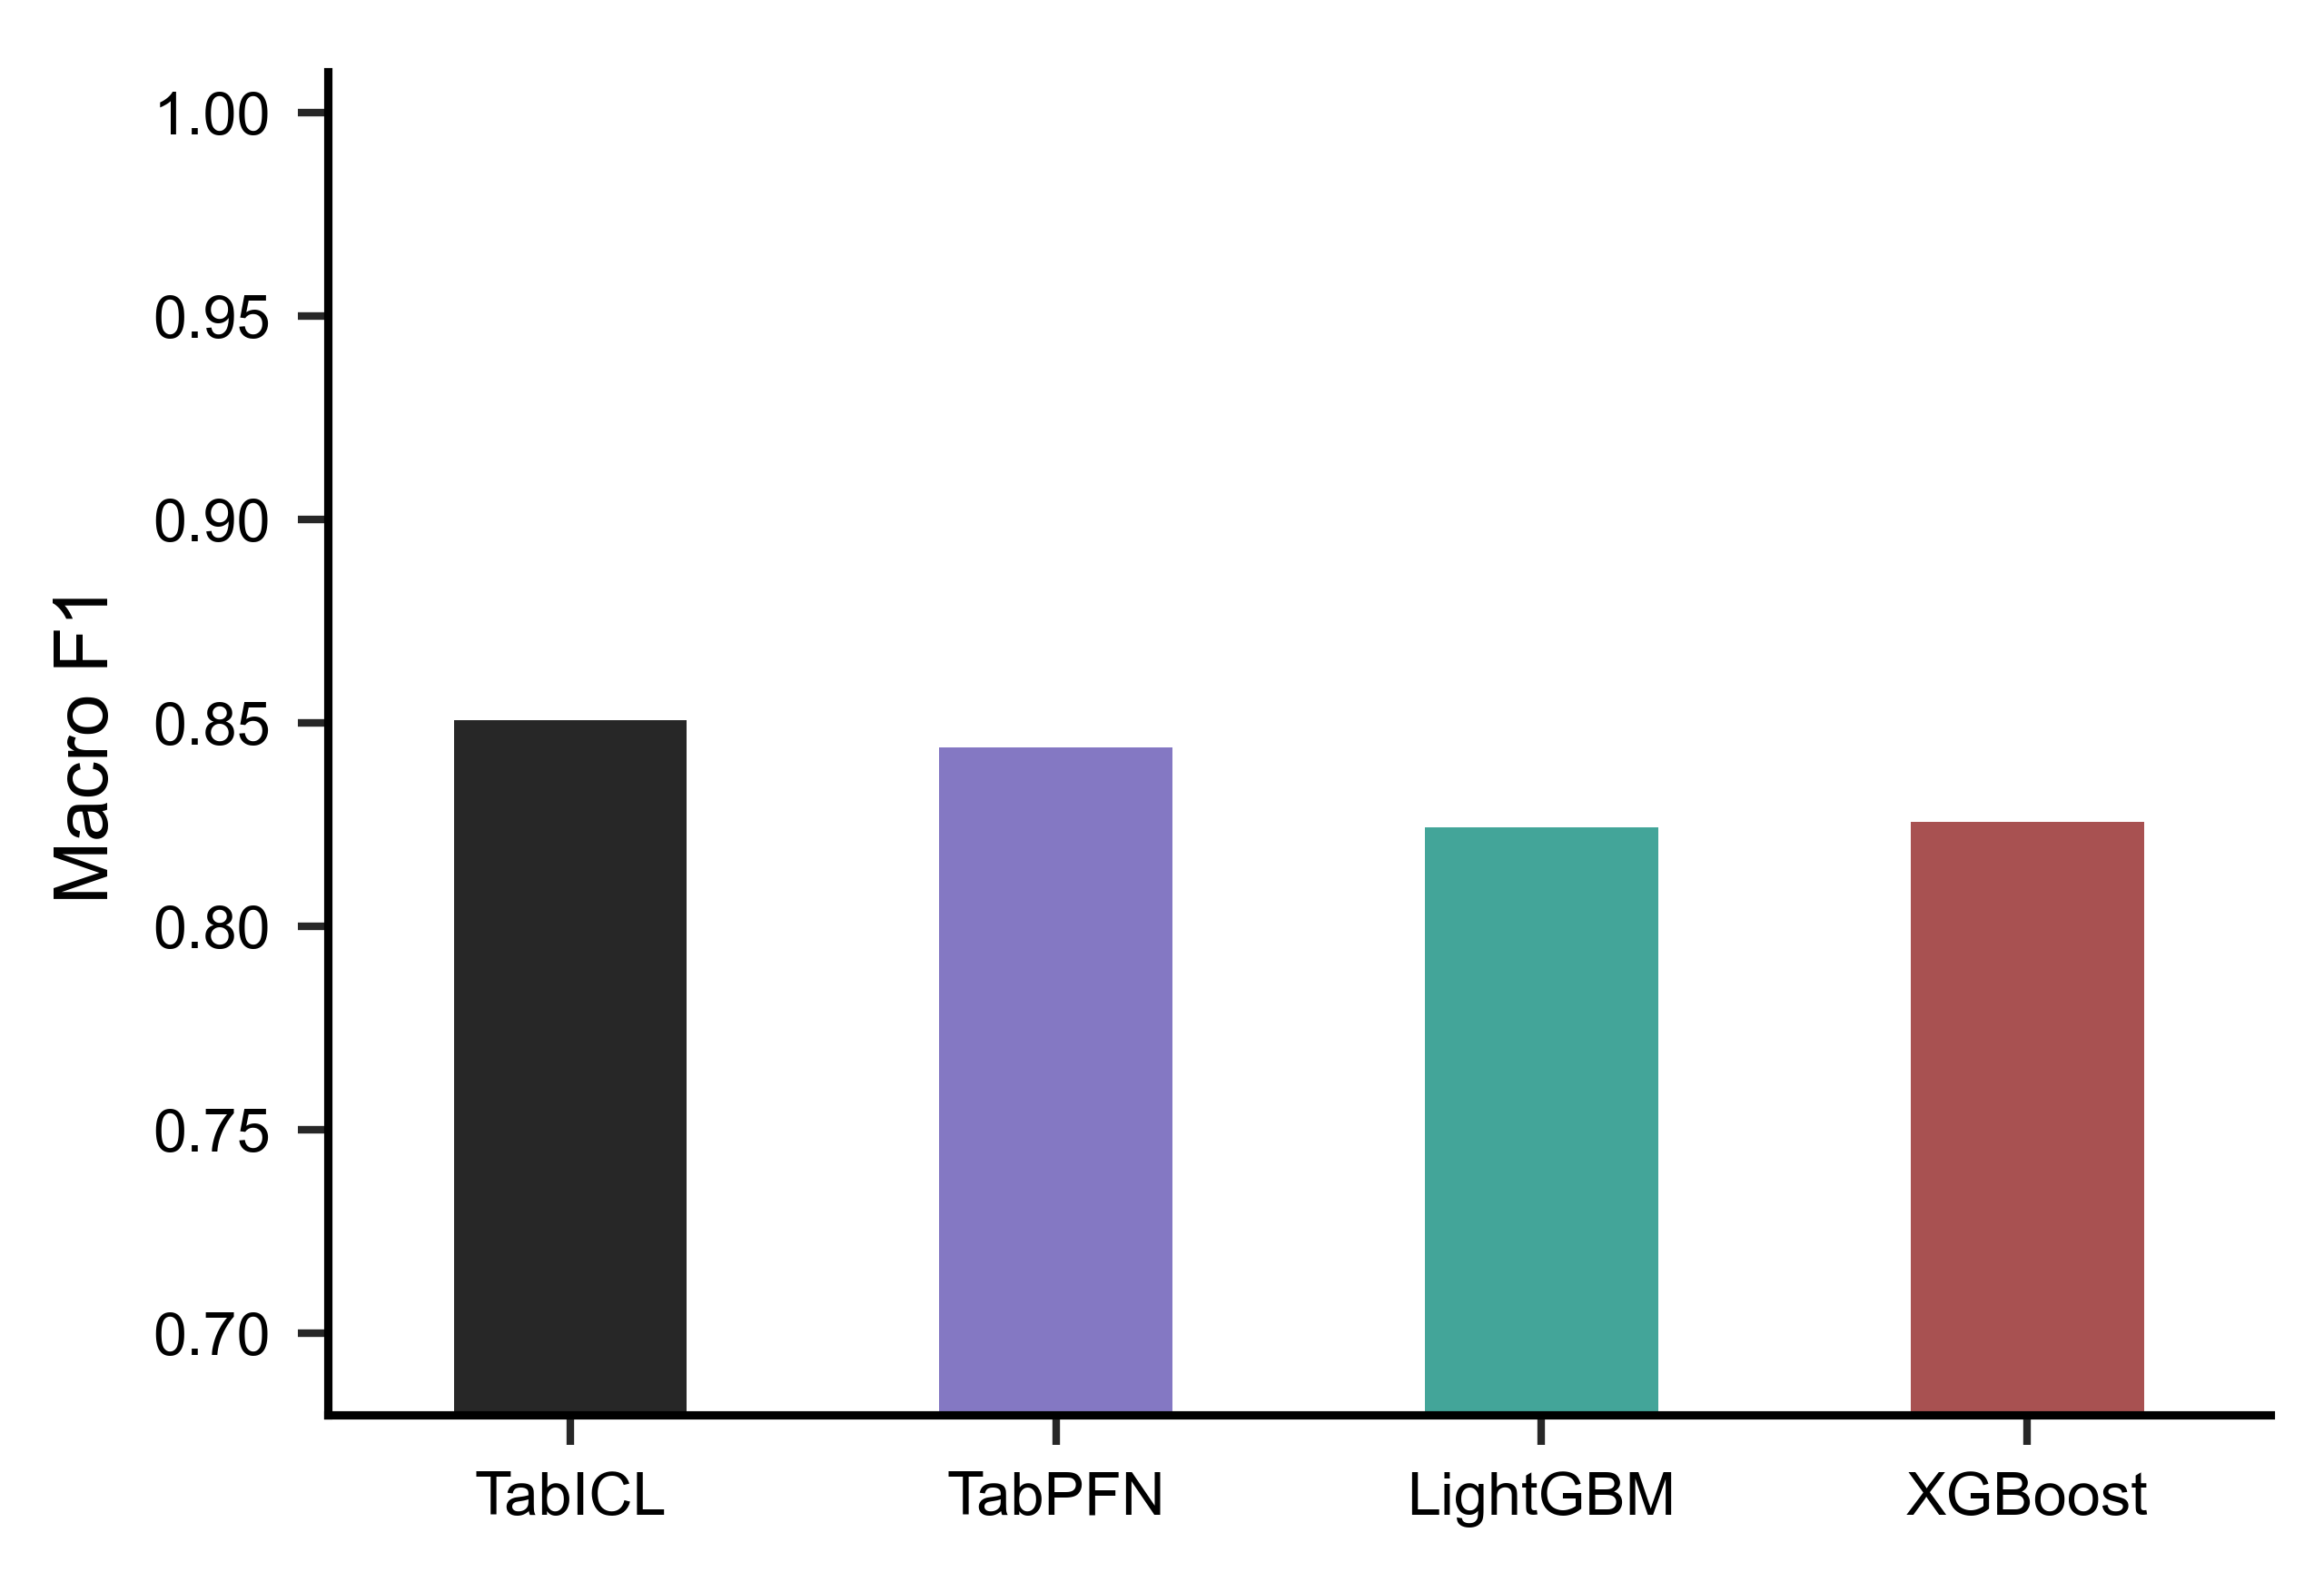
\includegraphics[width =.4\textwidth]{figures/performance_macro_f1_by_model.png}
    \caption{Prediction Performance}
    \label{fig: macro_f1}
\end{figure}


Both TabICL and TabPFN outperform baselines on average, with TabICL holding a consistent edge over TabPFN. However, \autoref{fig: macro_f1_by_dataset} shows advantage of TFMs is not uniform across datasets. On strongly separable binary tasks such as sylvine and ringnorm, all four models exceed 0.94 accuracy and the gaps between them are negligible. The advantage of TFM is most pronounced in the mfeat series, particularly the mid-dimensional variants (zernike, fourier, karhunen), where TabICL improves Macro-F1 by 5-12 percentage points over LightGBM. On the largest binary datasets (jm1, default\_of\_credit\_card\_clients), all models struggle similarly, with accuracy clustering tightly around 0.81–0.83 and Balanced Accuracy below 0.67, reflecting heavy class imbalance rather than model weakness.

\begin{figure}[H]
    \centering
    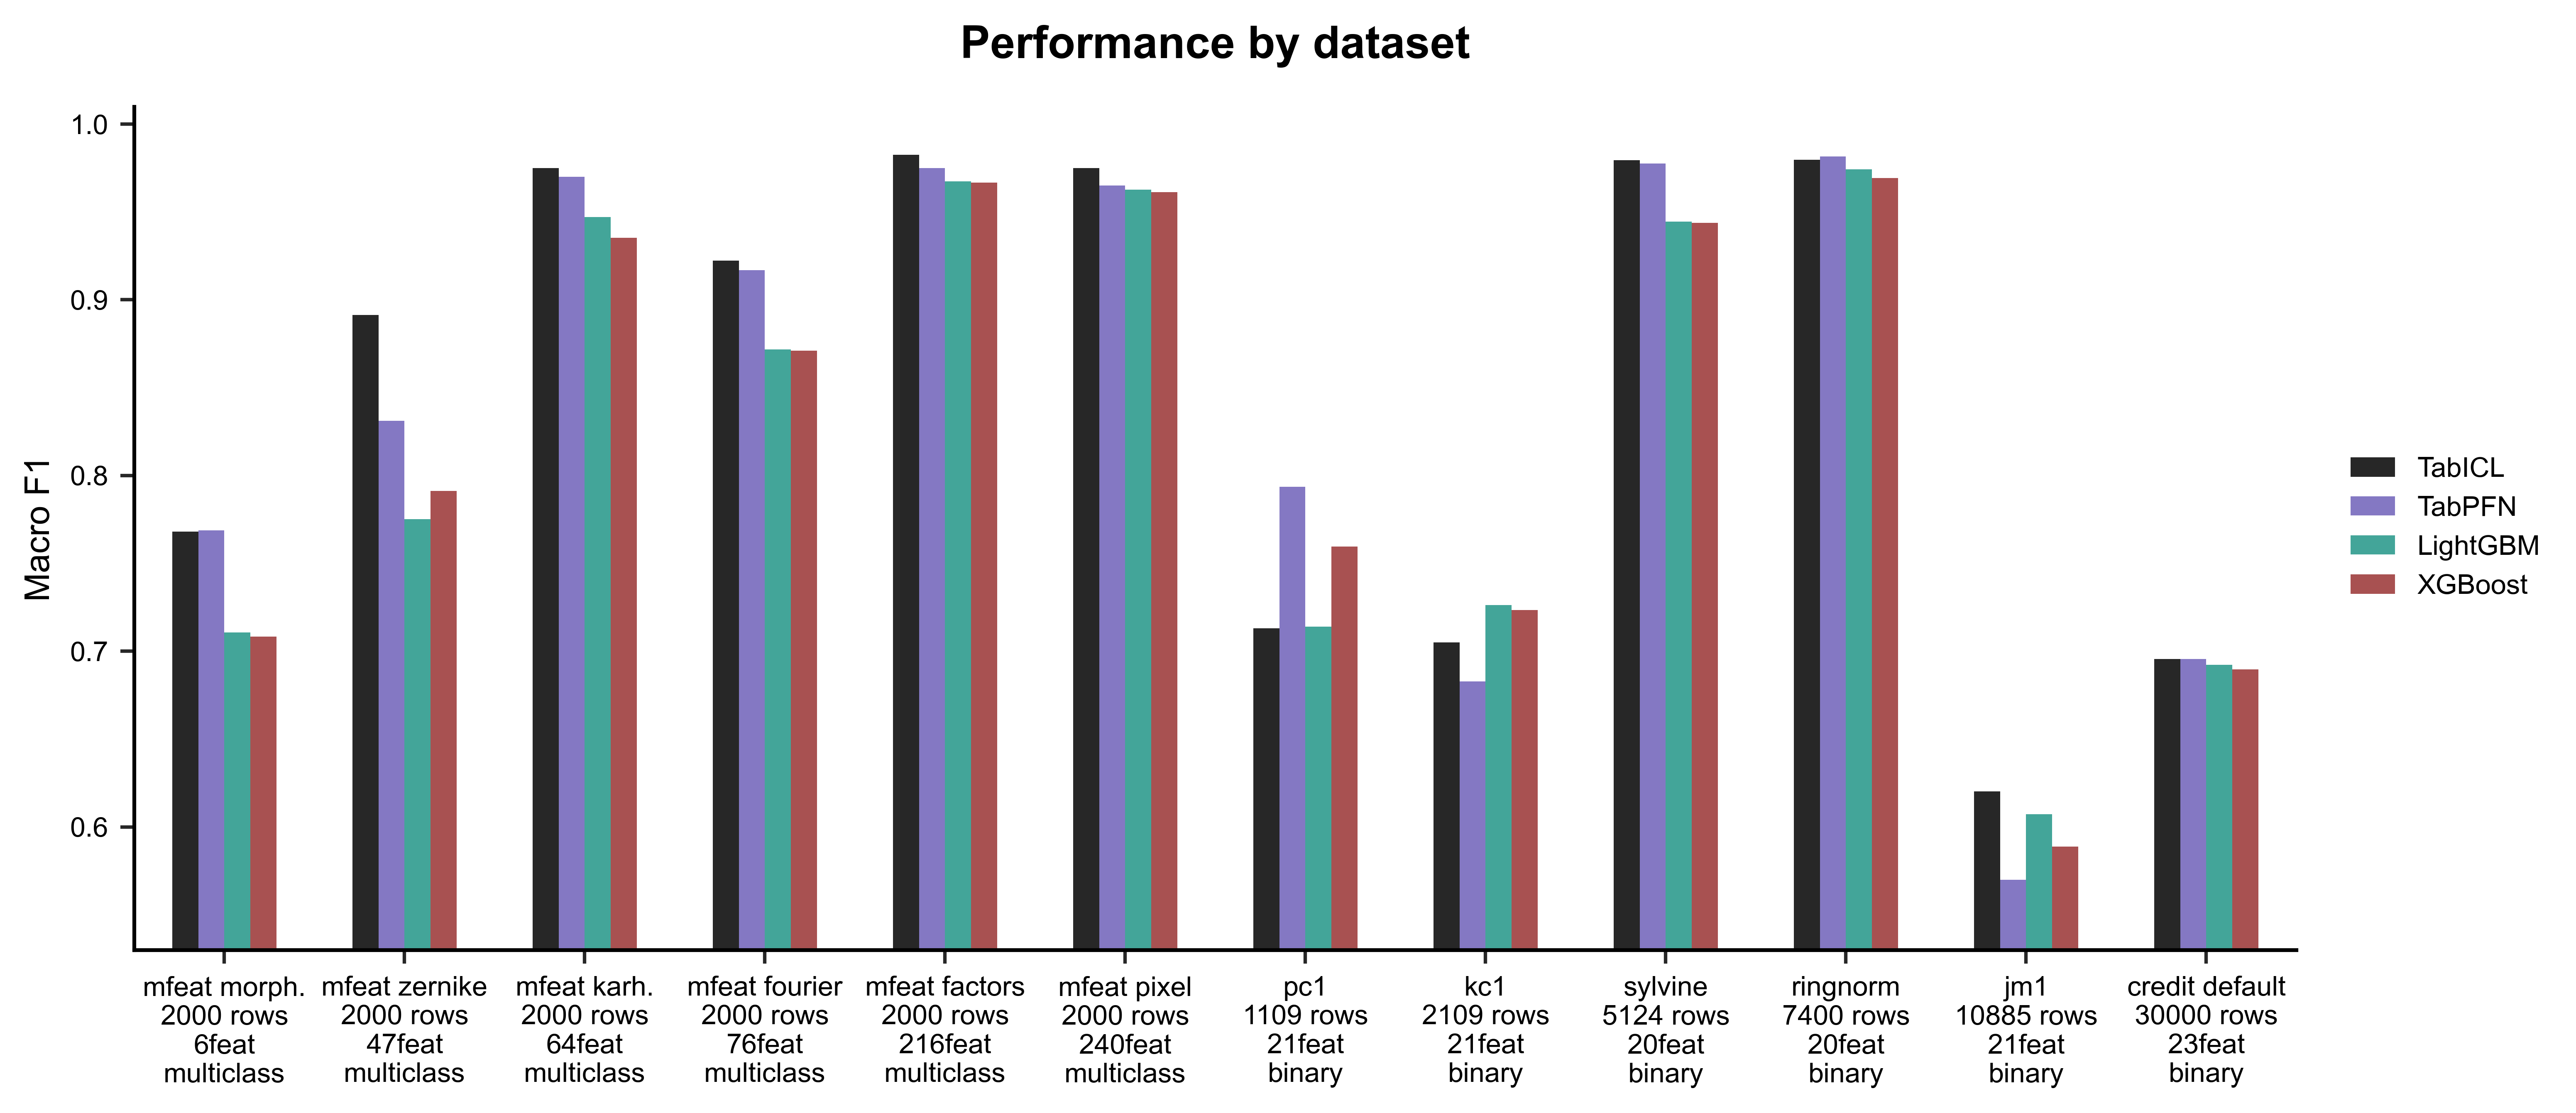
\includegraphics[width=0.5\linewidth]{figures/performance_macro_f1_by_dataset.png}
    \caption{Performance by Dataset}
    \label{fig: macro_f1_by_dataset}
\end{figure}


\textbf{Takeaway:} TFMs deliver better average predictive performance, but their advantage is concentrated on medium-complexity multi-class tasks. On easy or severely imbalanced binary tasks, tree baselines are nearly indistinguishable.


%%=======================




\subsection{Sample-Size Scalability}

To understand how model behavior evolves with data volume, we compare performance and cost across the six sample-scale datasets, ranging from 1,109 to 30,000 training samples.

\textbf{Performance trend:} \autoref{fig: sample_scale_macro_f1_line} plots Macro-F1 against increasing sample size. All four models improve as sample size grows from 1k to 5k, but the trajectory flattens or declines beyond 10k, particularly on jm1 and default\_of\_credit\_card\_clients where class imbalance penalizes Macro-F1 despite stable accuracy. TabICL maintains the highest Macro-F1 at every scale point.

\begin{figure}[H]
    \centering
    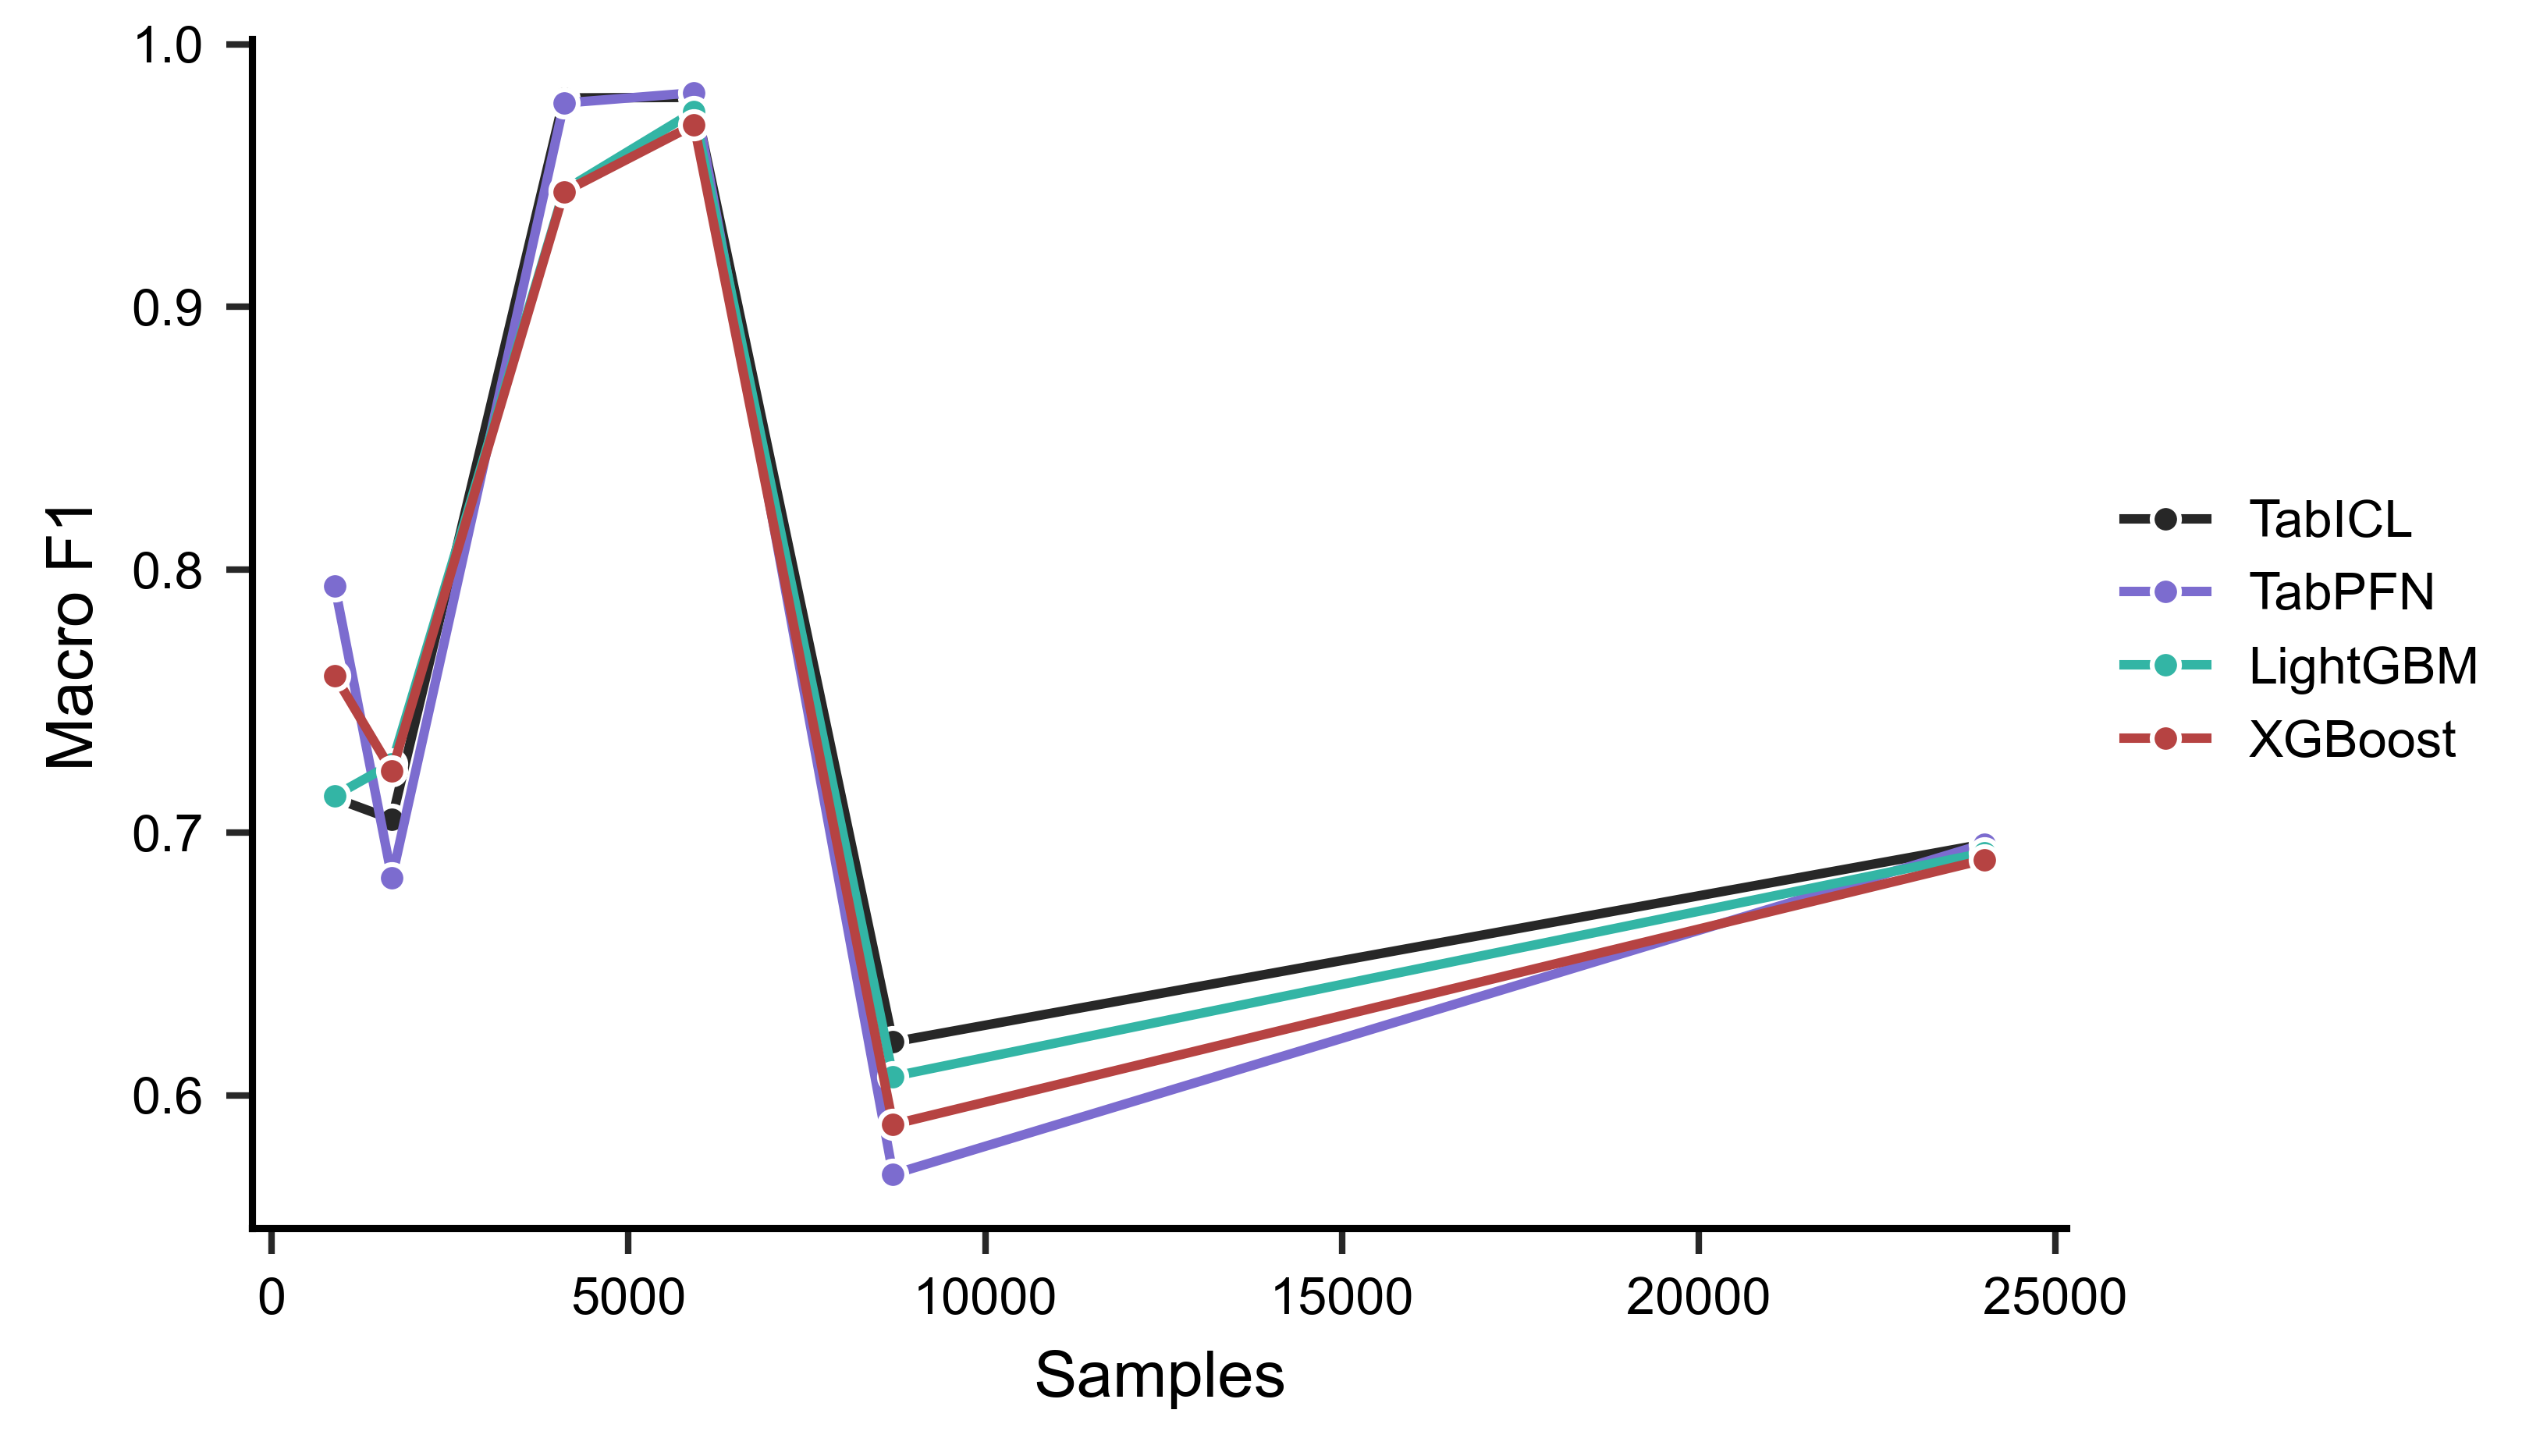
\includegraphics[width=0.5\linewidth]{figures/sample_scale_macro_f1_line.png}
    \caption{Macro-F1 Sample Scaling}
    \label{fig: sample_scale_macro_f1_line}
\end{figure}



%%=======================%%


\textbf{Time cost:} The more consequential divergence emerges in time cost. Figure X shows predict time on a log-log scale. As sample size increases from about 1k to 30k, LightGBM's predict time grows from 3 ms to 22 ms on a gaming laptop, and XGBoost from 2 ms to 5 ms. In contrast, TabPFN's predict time rises from 7 seconds to over 4,000 seconds, and TabICL's from 2 seconds to over 600 seconds. This is captured quantitatively by the scalability exponent $\alpha$, estimated via log-log linear regression:

\begin{figure}[H]
    \centering
    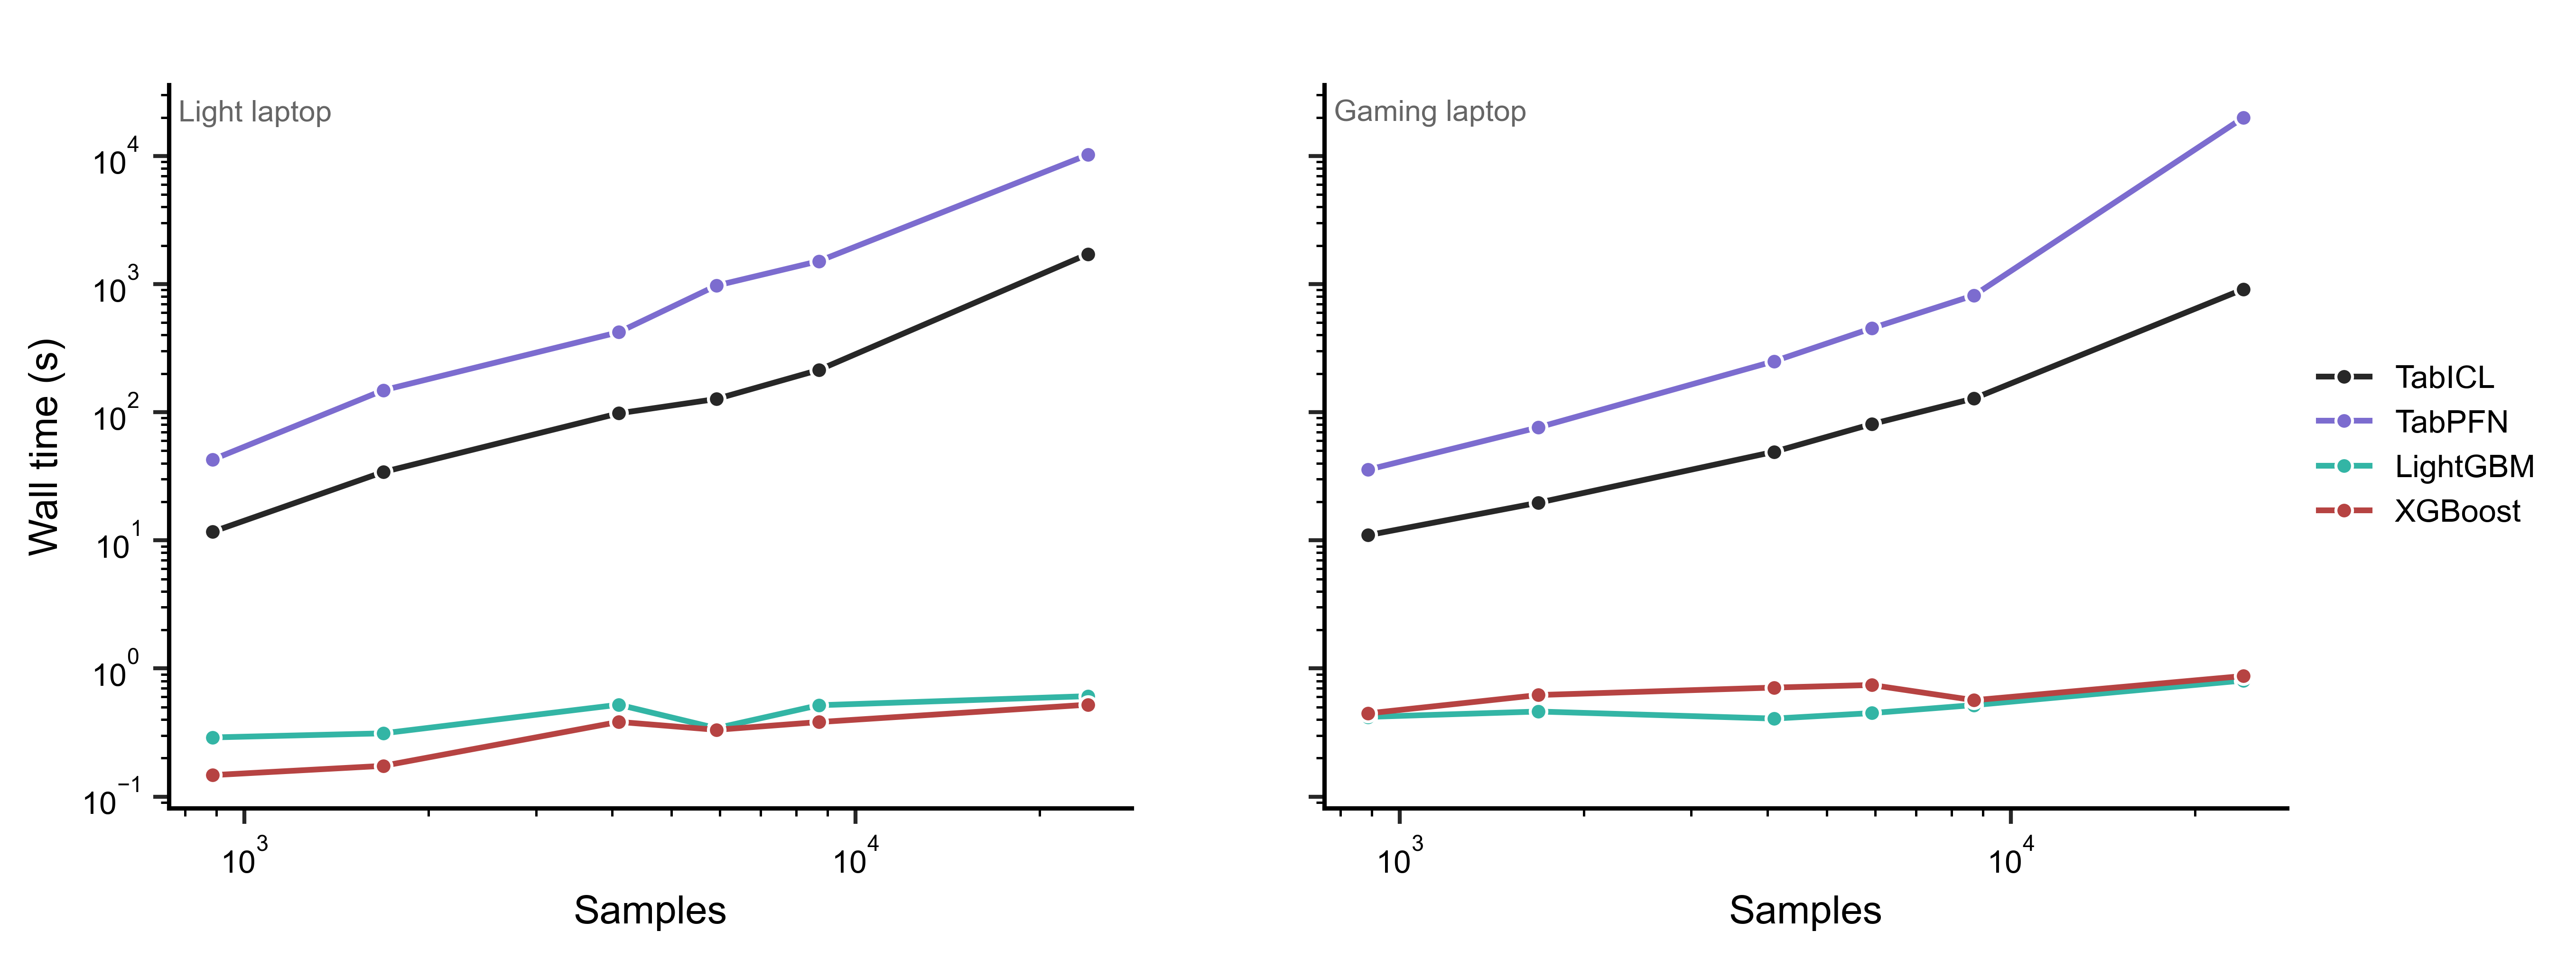
\includegraphics[width=0.5\linewidth]{figures/sample_scale_loglog_time.png}
    \caption{Time Cost Sample Scaling}
    \label{fig:placeholder}
\end{figure}

\begin{table}[H]
    \centering
    \begin{tabular}{ccc}
    \hline
         Model & $\alpha$ (predict\ time, Gaming) & $\alpha$ (predict\ time, Light) \\
    \hline
         LightGBM & 0.45 & 0.70 \\
         XGBoost & 0.37 & 0.30 \\
         TabICL & 1.41 & 1.50 \\
         TabPFN & 1.64 & 1.65 \\
    \hline
    \end{tabular}
    \caption{$\alpha$ Comparison\ on\ Sample\ Sizes}
    \label{tab: sample-size-related-time-cost}
\end{table}



\begin{figure}[H]
    \centering
    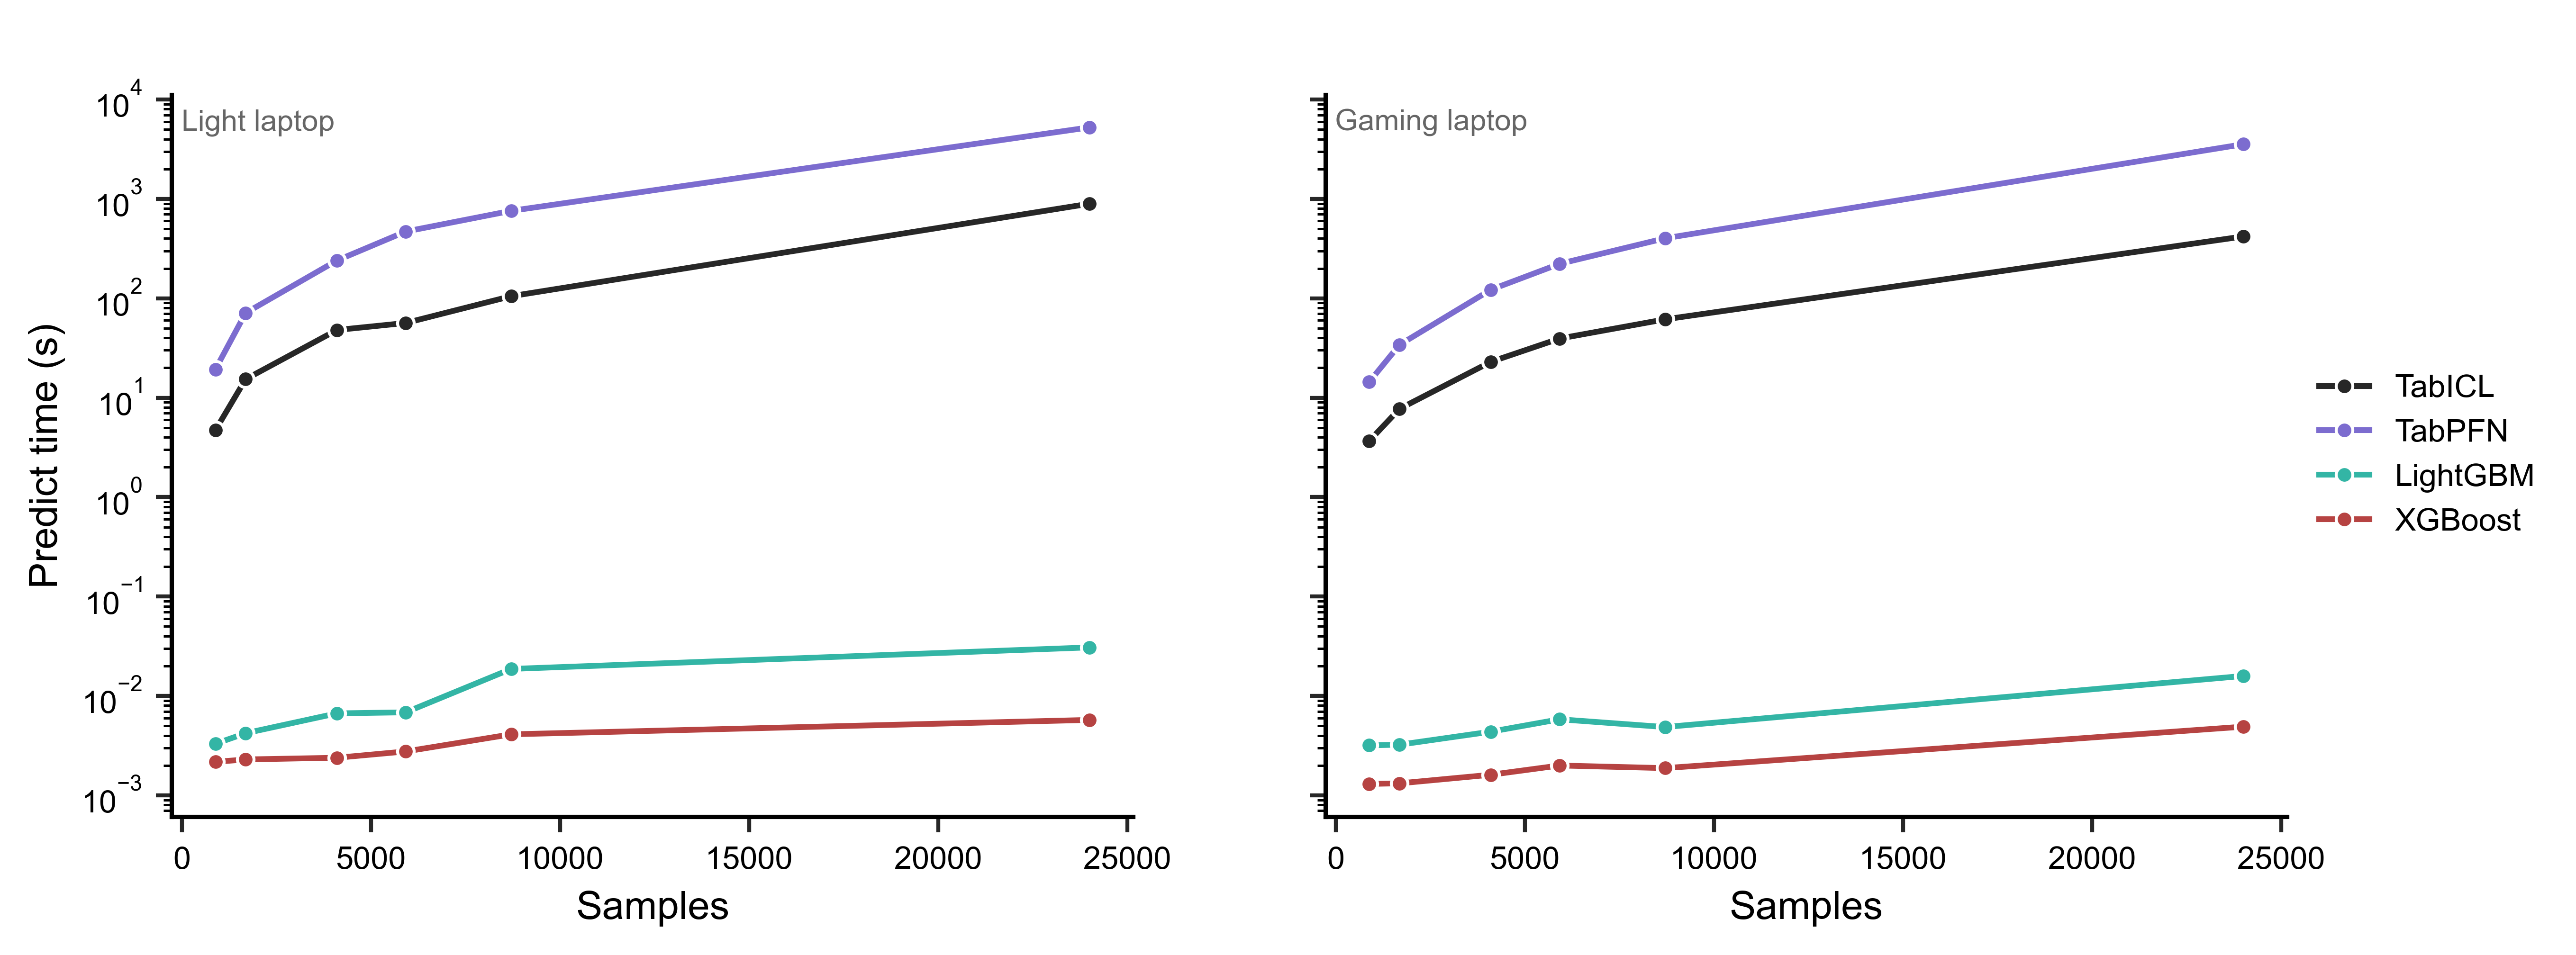
\includegraphics[width=0.5\linewidth]{figures/sample_scale_predict_time_seconds_line_by_device.png}
    \caption{Sample Scaling}
    \label{fig: sample_scale_prediction_time_seconds_line_by_device}
\end{figure}


An exponent near 1.0 indicates approximately linear growth; near 2.0 suggests quadratic behavior. TabPFN's $\alpha \approx 1.6$ indicates substantially super-linear time growth with sample size, meaning that doubling the number of training samples more than triples the predict time. TabICL fares slightly better at $\alpha \approx 1.4 \sim 1.5$, but both are far above the tree baselines ($\alpha \approx 0.3 \sim 0.7$). LightGBM and XGBoost scale sub-linearly with respect to sample size in predict time.



%%=======================%%


\textbf{Memory cost:} Peak memory follows a similar pattern. Tree baselines remain nearly flat at 150–250 MB regardless of sample size, while TabICL grows from $\approx$ 1.4 GB on \texttt{pc1} to $\approx$ 18.8 GB on default\_of\_credit\_card\_clients (gaming laptop), and TabPFN from 1.0 GB to 4.8 GB. The $\alpha$ values for memory growth confirm this: TabICL $\alpha \approx 0.76\sim 0.84$, TabPFN $\alpha \approx 0.43$, tree models $\alpha \approx 0.02 \sim 0.04$.


\begin{figure}[H]
    \centering
    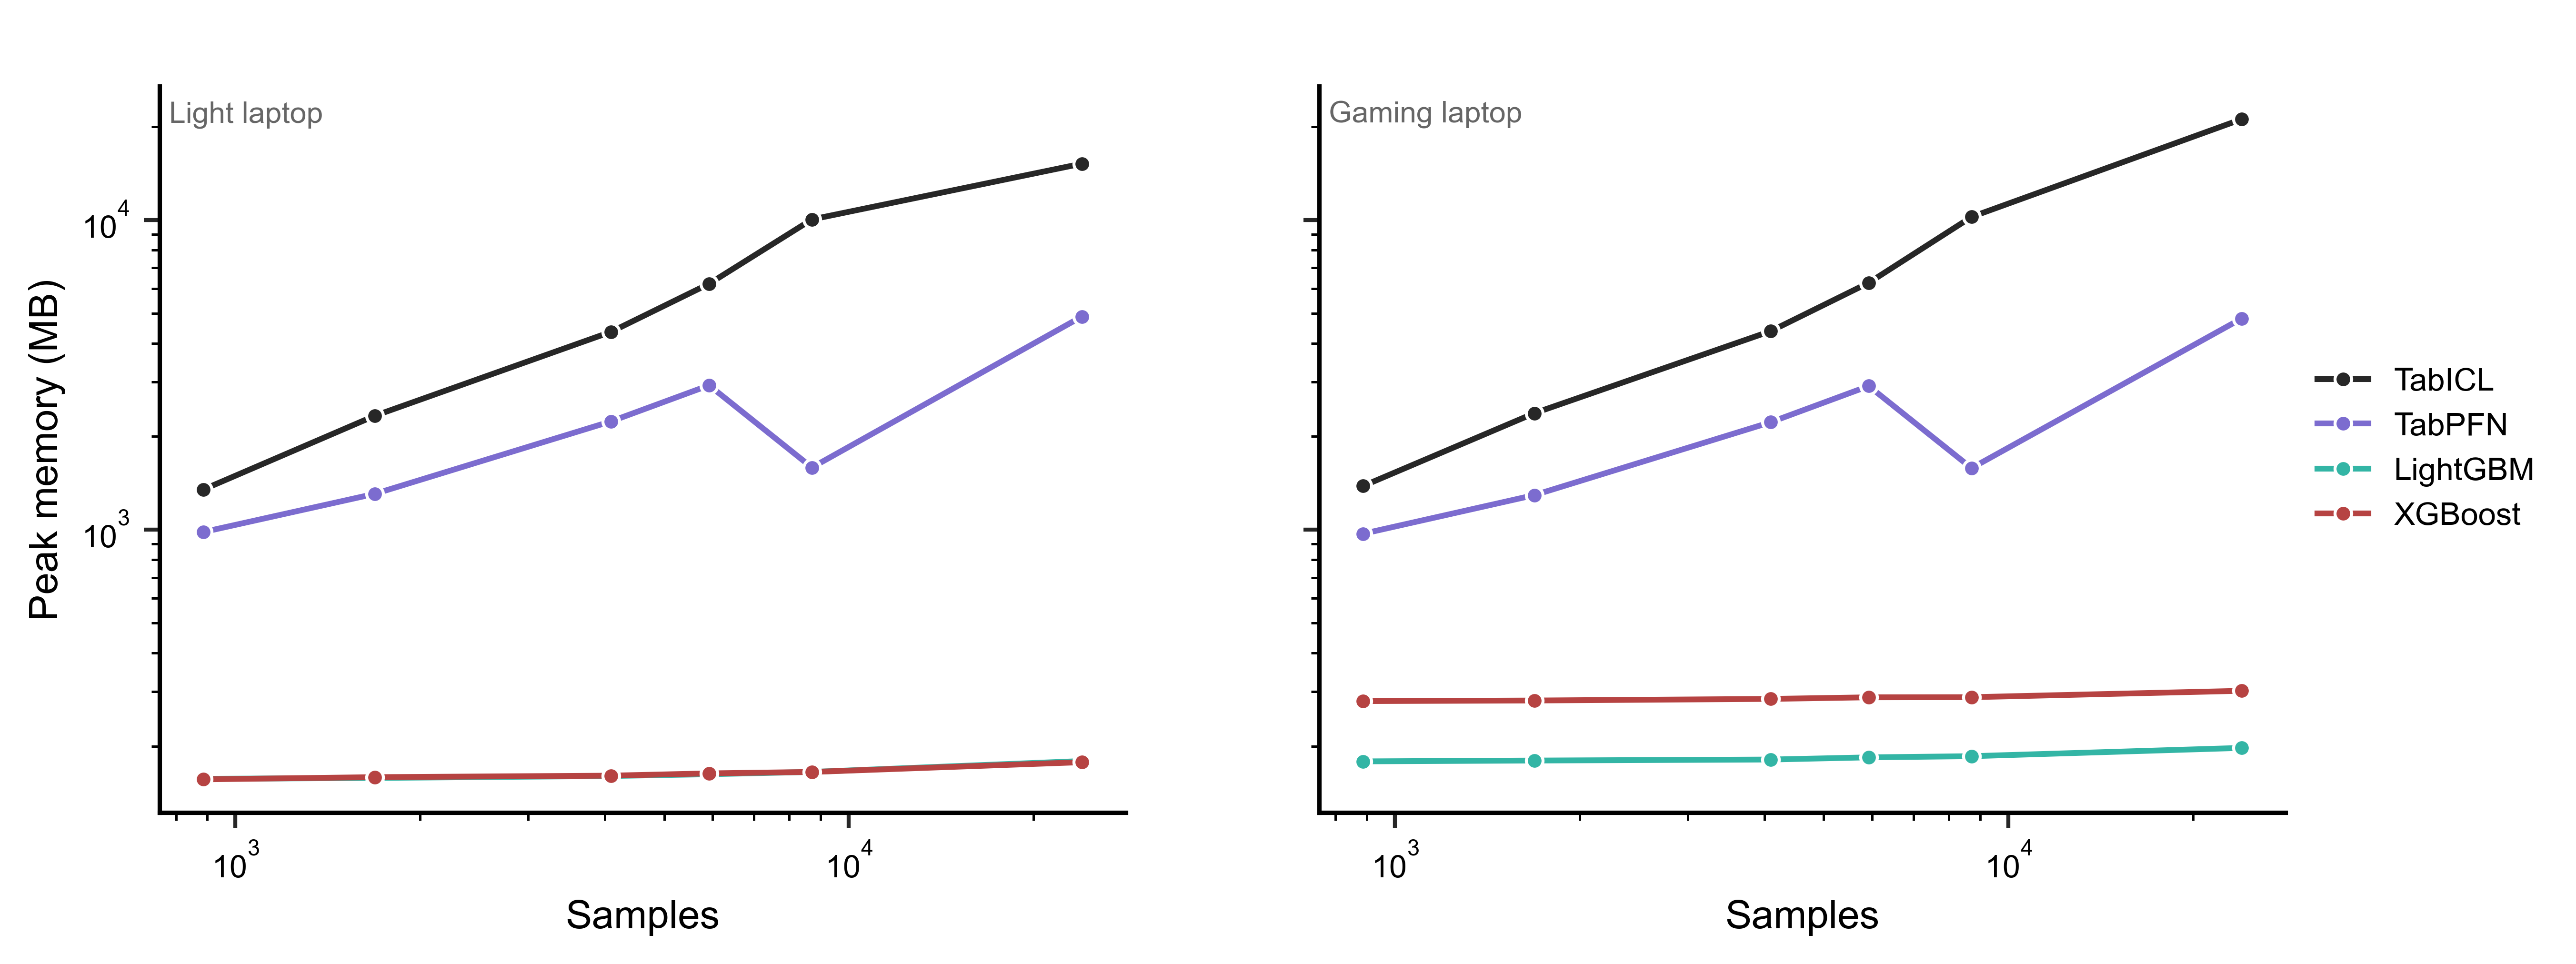
\includegraphics[width=0.5\linewidth]{figures/sample_scale_loglog_memory.png}
    \caption{Memory Sample Scaling}
    \label{fig: sample_scale_loglog_memory}
\end{figure}



\textbf{Takeaway:} TFMs maintain their predictive advantage across sample sizes, but pay a steep and growing computational cost as data volume increases. For tasks above 10k samples on CPU, the practical runtime of TFMs may become prohibitive.


%%=======================%%


\subsection{Feature-Count Scalability}

We now examine the second controlled-variable line: six mfeat datasets with identical sample size (2,000 rows) but varying feature dimensionality from 6 to 240.


\textbf{Performance trend:} \autoref{fig: feature_scale_macro_f1_line} shows that Macro-F1 rises sharply with feature count for all models. On the low-dimensional mfeat-morphological (6 features), all models achieve only $\approx 0.71\sim 0.78$ Macro-F1. By mfeat-factors (216 features), performance exceeds 0.96, and by mfeat-pixel (240 features) it reaches $0.96\sim 0.97$. TabICL and TabPFN consistently outperform tree baselines across the mid-dimensional spectrum (zernike through karhunen), but the gap narrows at the highest dimensions as all models approach near-perfect accuracy.


\begin{figure}[H]
    \centering
    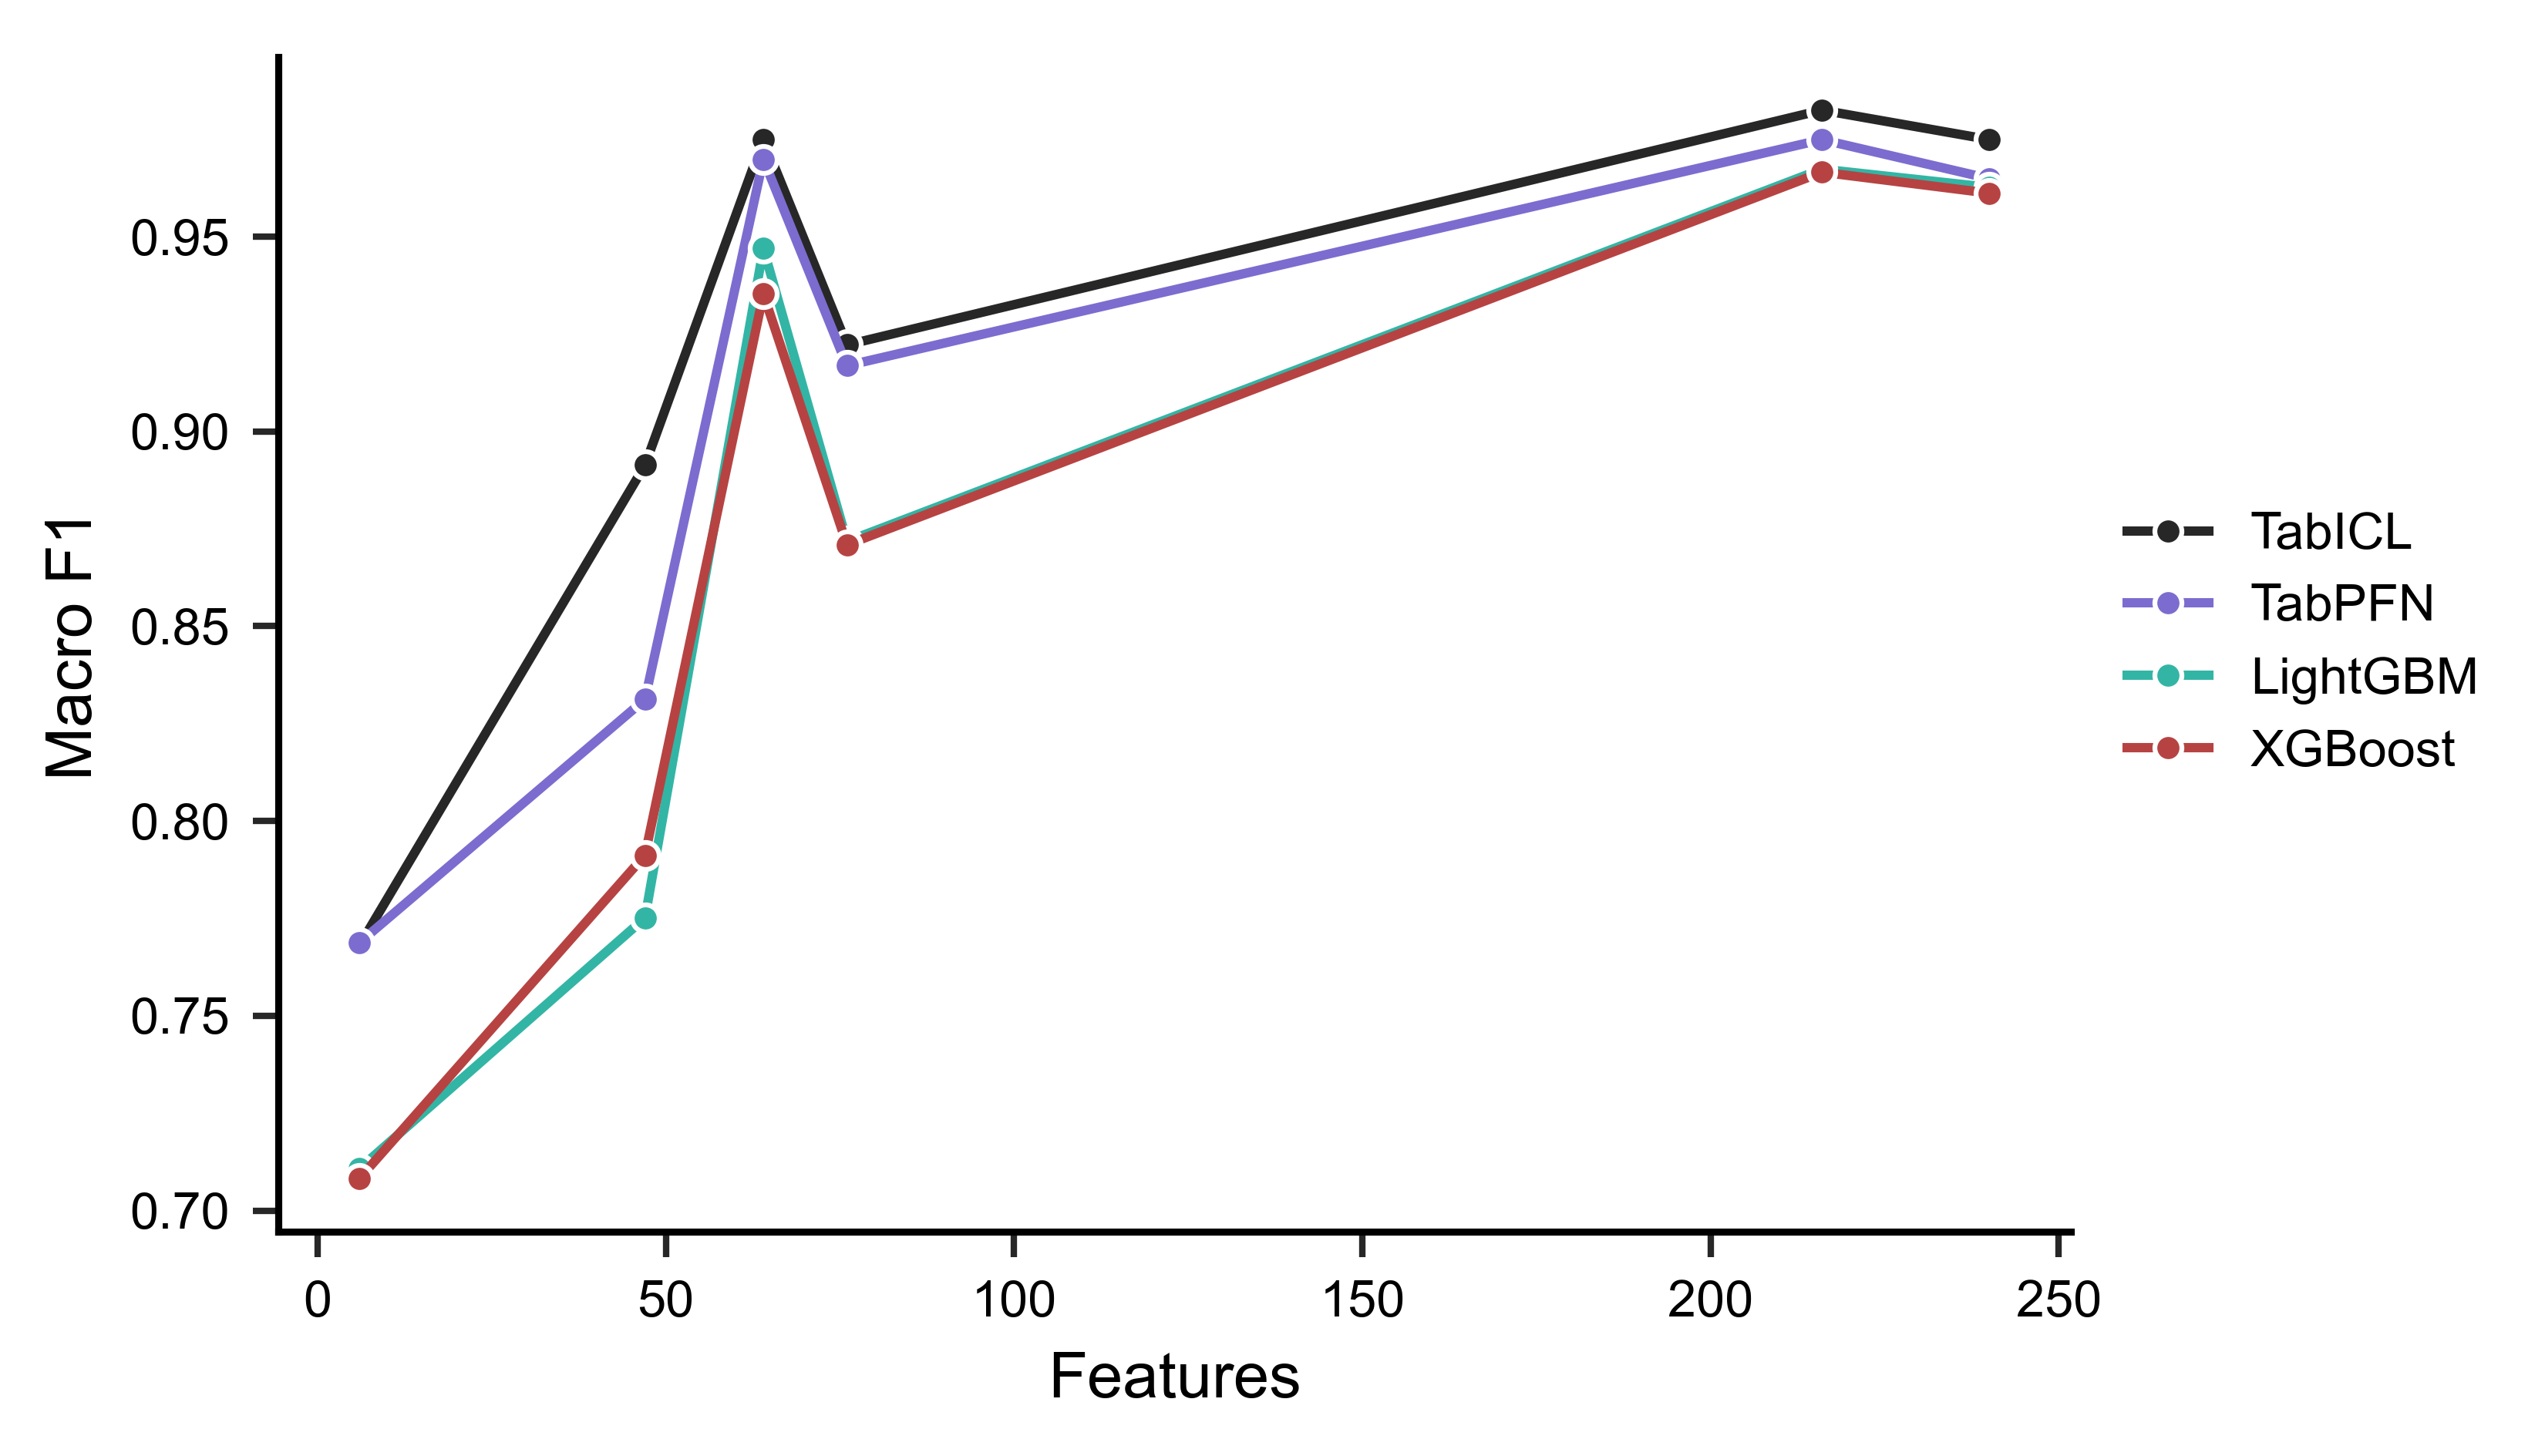
\includegraphics[width=0.5\linewidth]{figures/feature_scale_macro_f1_line.png}
    \caption{Feature Macro-F1 Scaling}
    \label{fig: feature_scale_macro_f1_line}
\end{figure}



\textbf{Time cost:} Feature count affects TFMs more than tree baselines. The measured α values for predict time versus feature count are:


\begin{table}[H]
    \centering
    \begin{tabular}{ccc}
    \hline
    Model & $\alpha$ (predict\ time, Gaming) & $\alpha$ (predict\ time, Light) \\
    \hline
    LightGBM  & 0.07 & -0.27 \\
    XGBoost & -0.01 & -0.09 \\
    TabICL & 0.68 & 0.69 \\
    TabPFN & 0.94 & 0.82 \\
    \hline
    \end{tabular}
    \caption{$\alpha$\ Comparison\ on\ Features}
    \label{tab: time_cost_feature}
\end{table}


\textbf{Scalability trend:} Notably, tree baselines show near-zero or negative $\alpha$ on feature-count scalability, indicating that their inference time is nearly independent of feature dimensionality in this regime. In contrast, both TFMs scale substantially with feature count: doubling the number of features approximately doubles the predict time for TabICL ($\alpha \approx 0.69$) and slightly more than doubles for TabPFN ($\alpha \approx 0.82\sim 0.94$). On \texttt{mfeat-pixel} (240 features, 2,000 samples), TabPFN predict time reaches 293 seconds on a gaming laptop, compared to 0.02 seconds for LightGBM—a four-order-of-magnitude difference.

\begin{figure}
    \centering
    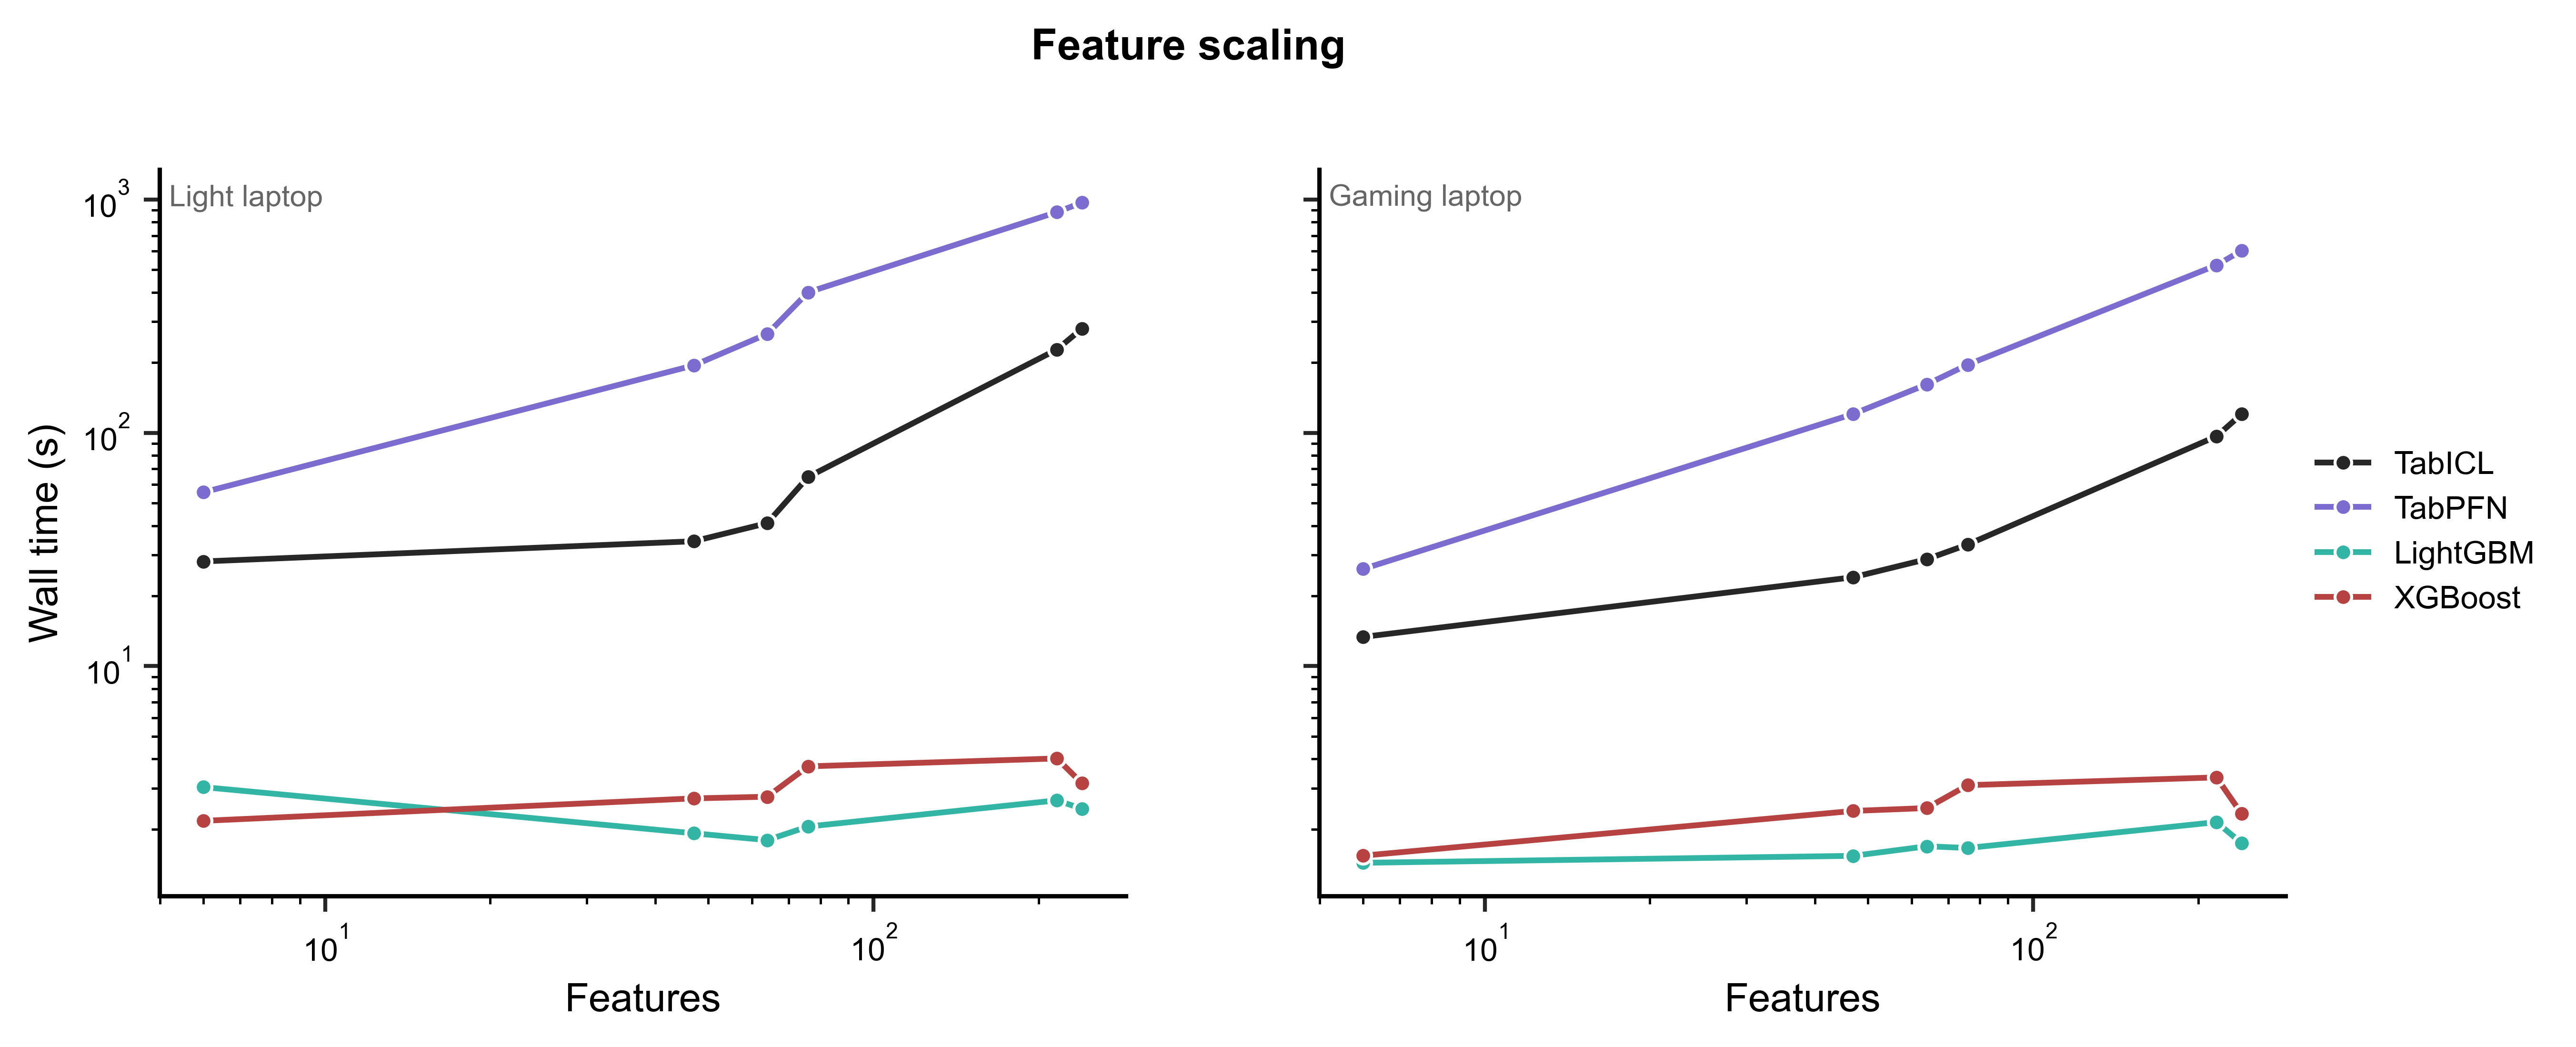
\includegraphics[width=0.5\linewidth]{figures/feature_scale_loglog_time.png}
    \caption{Enter Caption}
    \label{fig:placeholder}
\end{figure}


\textbf{Memory cost:} Memory scaling with feature count is less extreme than with sample size. TabICL memory grows from 1.2 GB (6 features) to 17.5 GB (240 features), while tree baselines remain at 190–250 MB throughout. TabPFN memory grows from 0.7 GB to 2.2 GB.

\begin{figure}
    \centering
    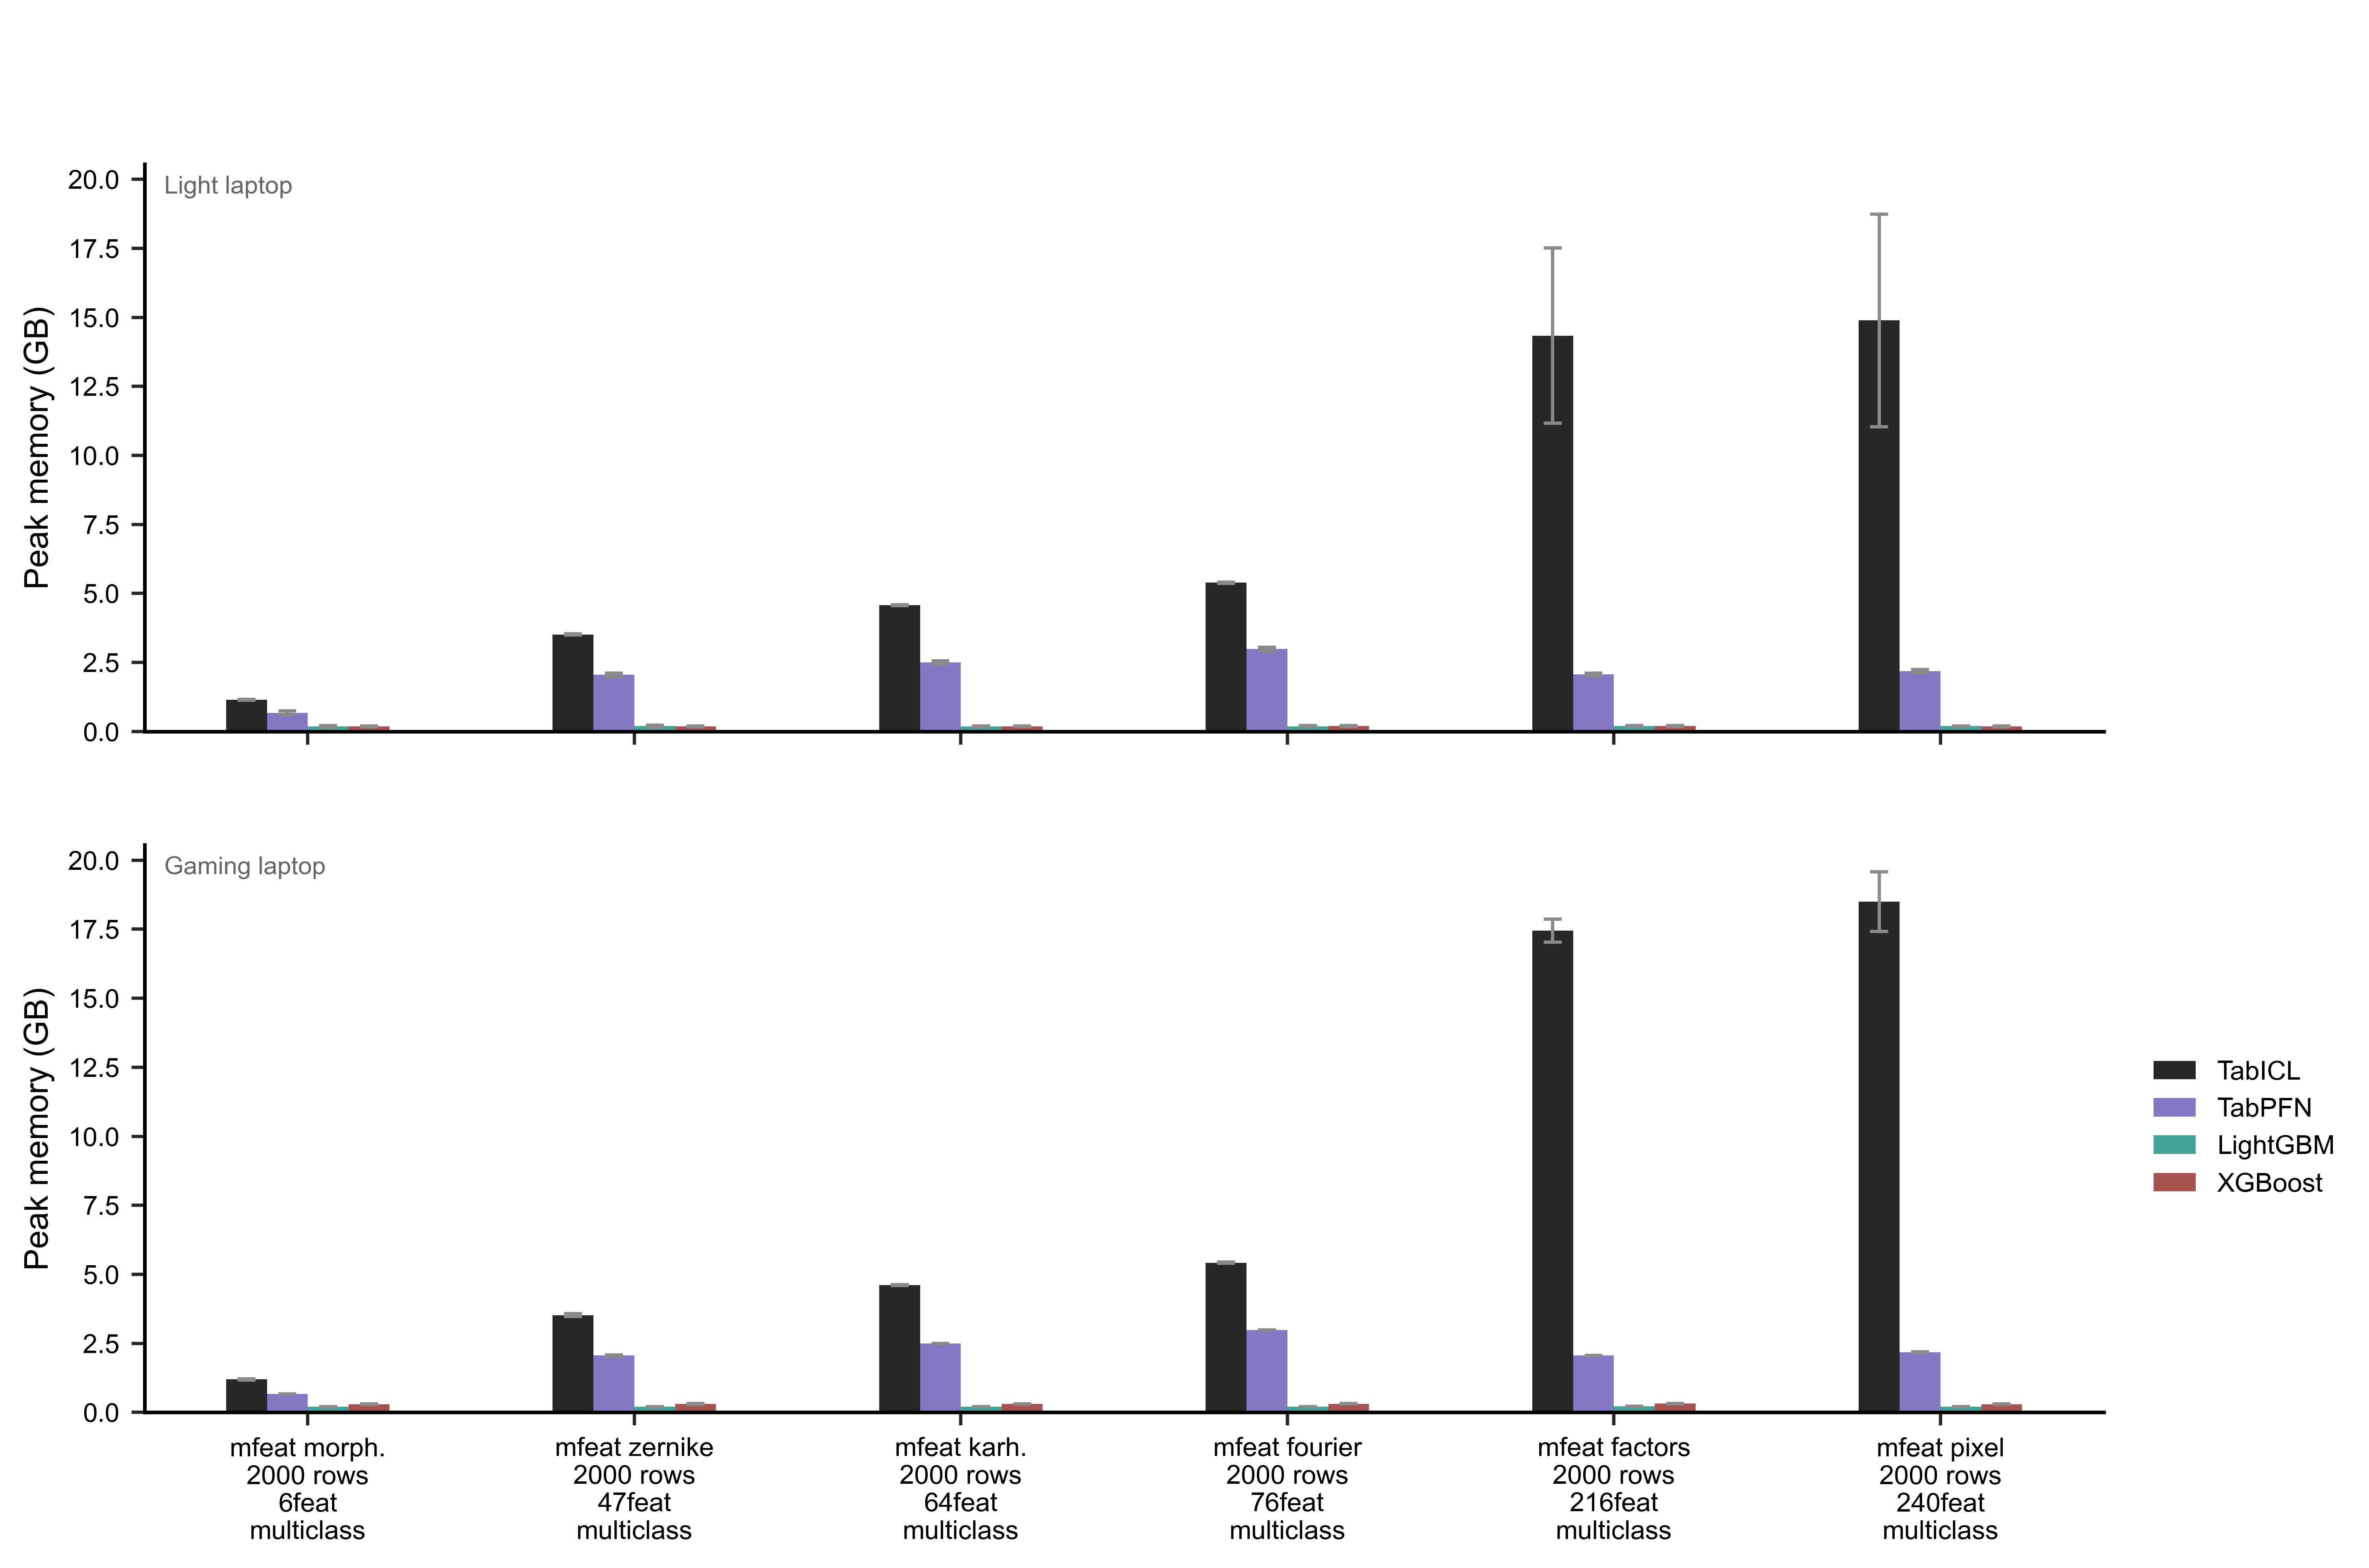
\includegraphics[width=0.5\linewidth]{figures/feature_scale_peak_memory_bar_by_device.png}
    \caption{Enter Caption}
    \label{fig:placeholder}
\end{figure}


\textbf{Takeaway:} Feature dimensionality has a modest impact on tree models but a substantial one on TFMs, particularly TabPFN. However, the absolute costs are far lower than for sample-size scaling—even at 240 features, the 2,000-sample \texttt{mfeat-pixel} runs in under 5 minutes for TabPFN, whereas 30,000 samples $\times$ 23 features requires over an hour. This suggests that feature count and sample count interact in determining TFM cost, but sample count dominates.


\subsection{Confidence Calibration}

Beyond predictive accuracy, we examine whether models can assess the reliability of their own predictions through confidence calibration. Figure X compares the mean confidence assigned to correct versus incorrect predictions for each model.
All four models assign substantially higher confidence to correct predictions than to incorrect ones, confirming that confidence carries signal about prediction quality. However, the degree of separation varies. TabICL and TabPFN exhibit the largest confidence gaps, exceeding 0.30 on several mfeat datasets—meaning that correct predictions are assigned confidence near 0.92–0.99 while wrong predictions receive around 0.54–0.65. In contrast, LightGBM and XGBoost produce narrower gaps: on mfeat-morphological, LightGBM's confidence gap is 0.05 (correct mean 0.95 vs. wrong mean 0.90), meaning the model remains highly confident even when mistaken.
A concerning pattern emerges across all models: wrong predictions routinely receive non-trivial confidence. On the binary dataset jm1, LightGBM assigns a mean confidence of 0.76 to its errors, and TabPFN assigns 0.76. Even TabICL, which shows the best overall separation, assigns 0.76 to wrong predictions on the same dataset. This indicates that none of the models provide a reliable "I don't know" signal—incorrect predictions are not accompanied by low confidence.
Takeaway: Confidence scores are directionally useful (correct > wrong) for all models, but the absolute calibration is poor. Users should not interpret high confidence as a guarantee of correctness, regardless of the model family.

\begin{figure}[H]
    \centering
    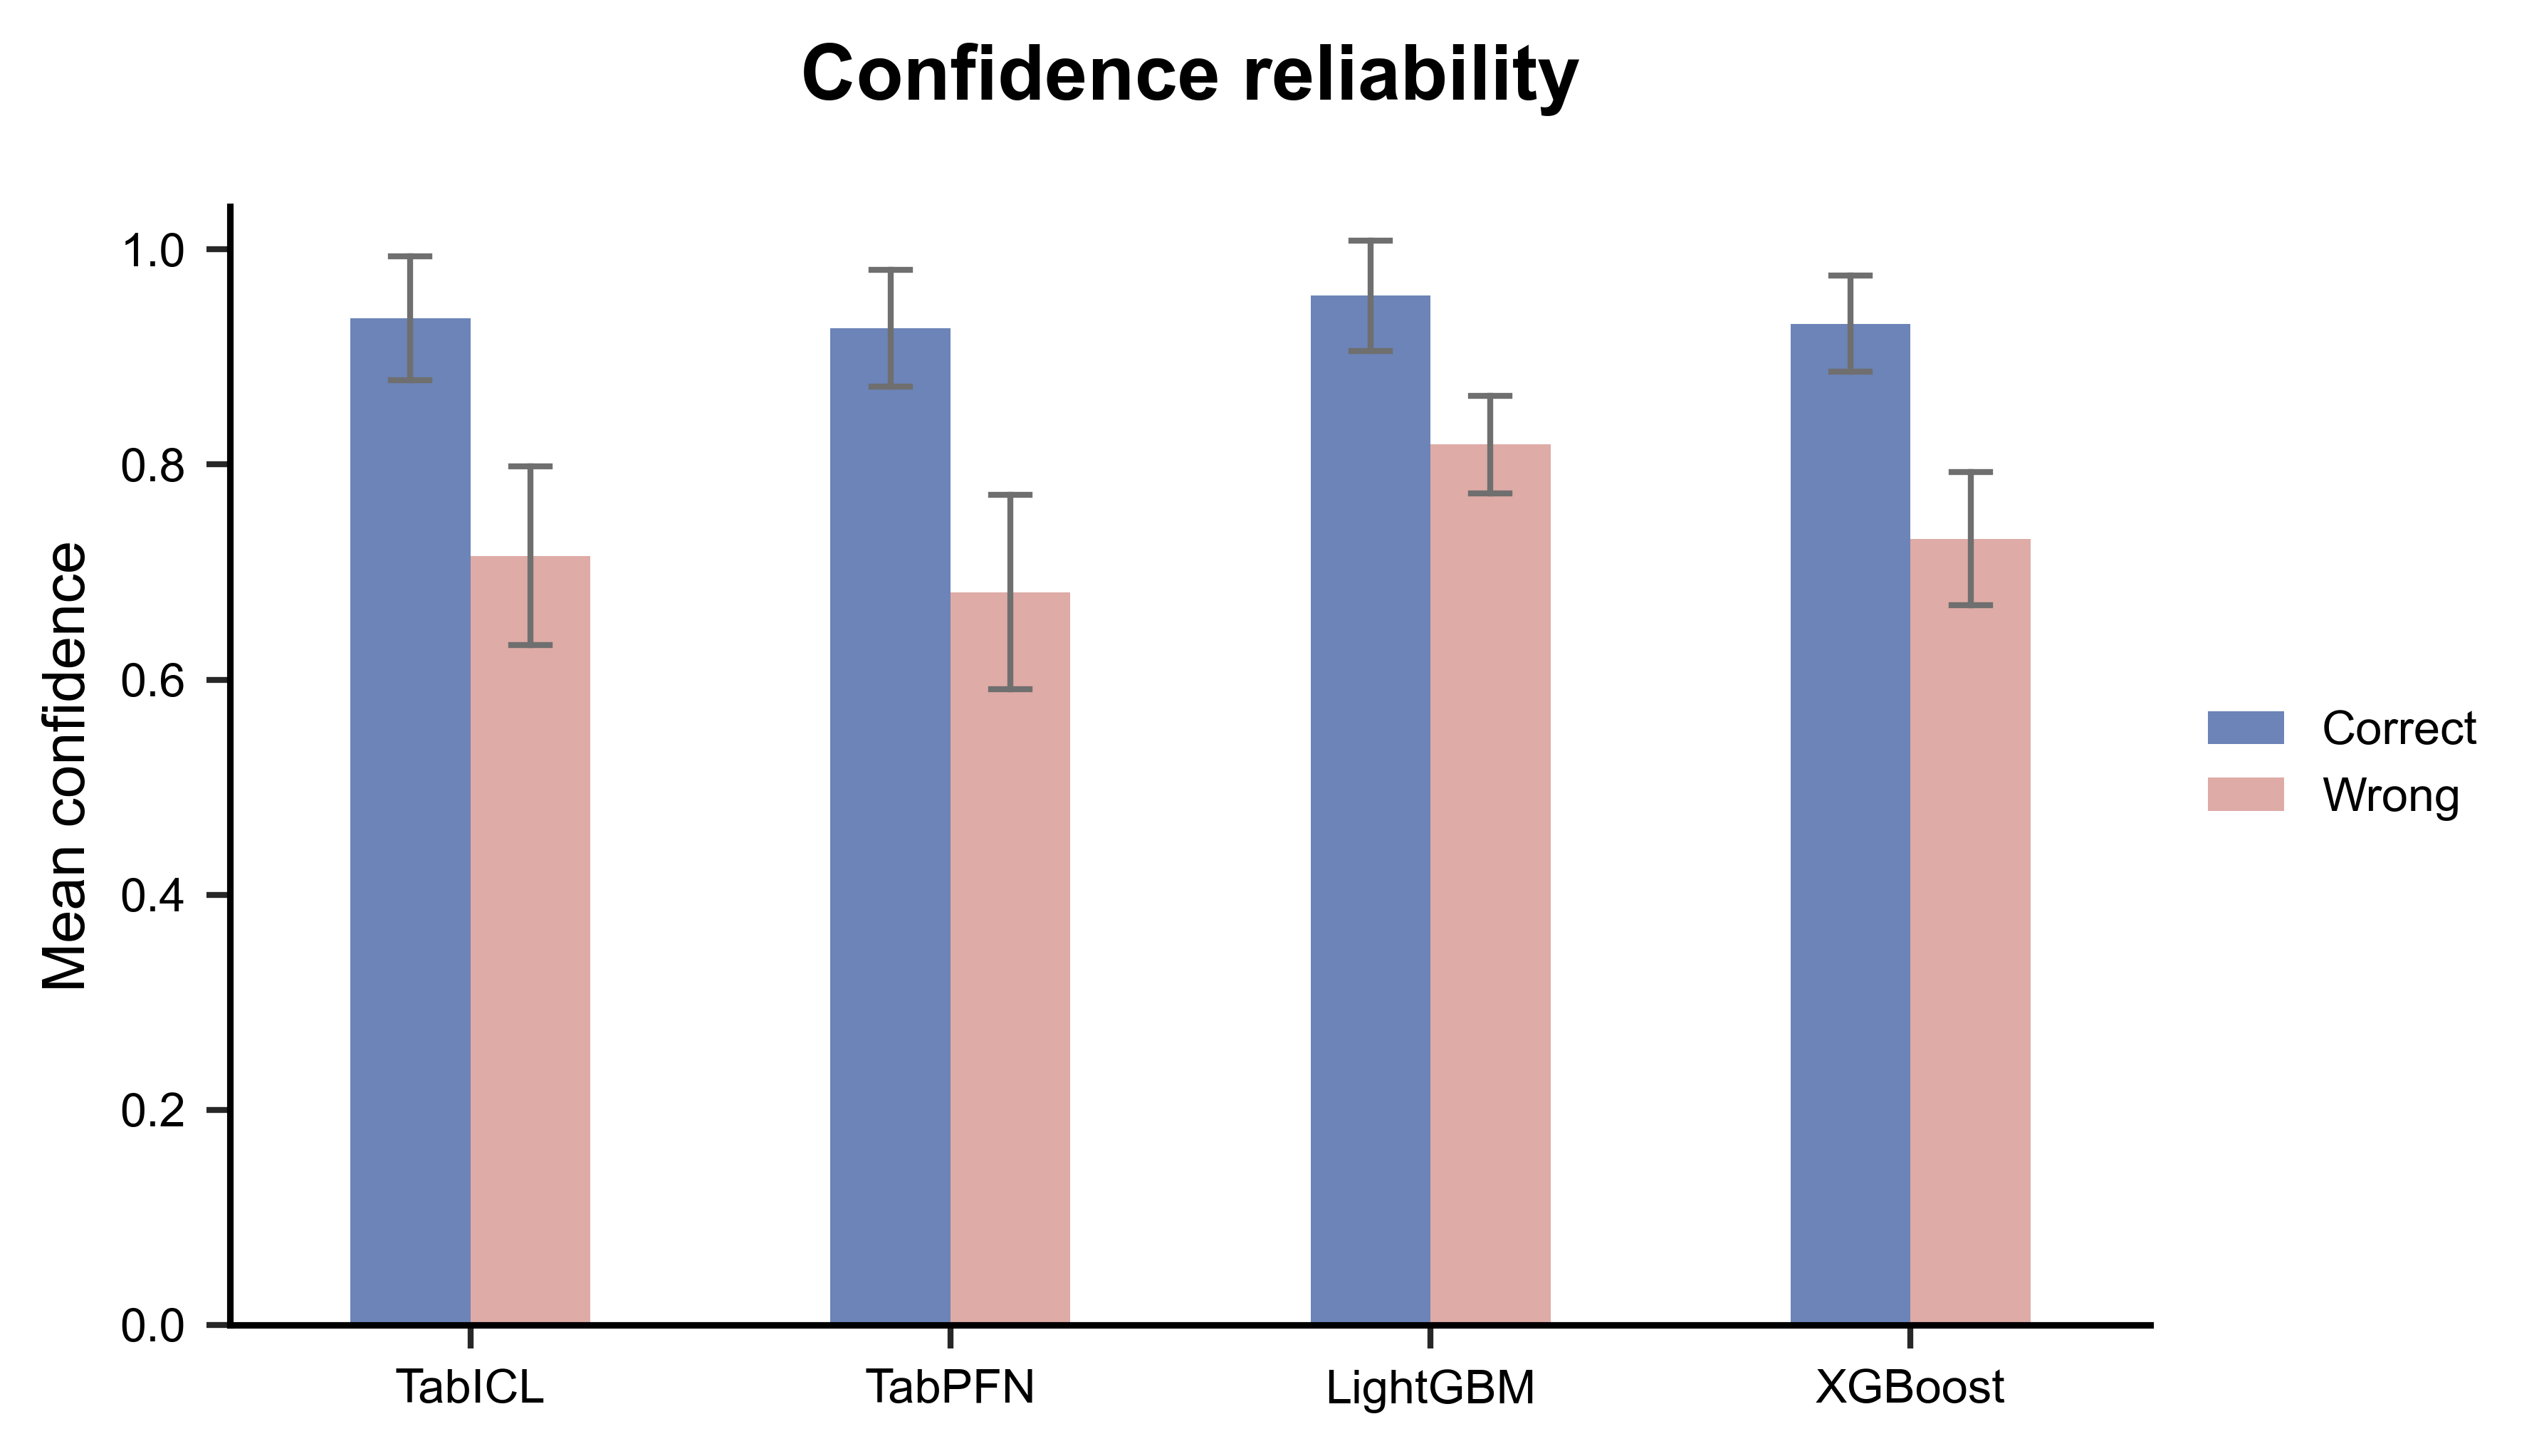
\includegraphics[width=0.5\linewidth]{figures/confidence_correct_vs_wrong.png}
    \caption{Enter Caption}
    \label{fig:placeholder}
\end{figure}


\begin{figure}[H]
    \centering
    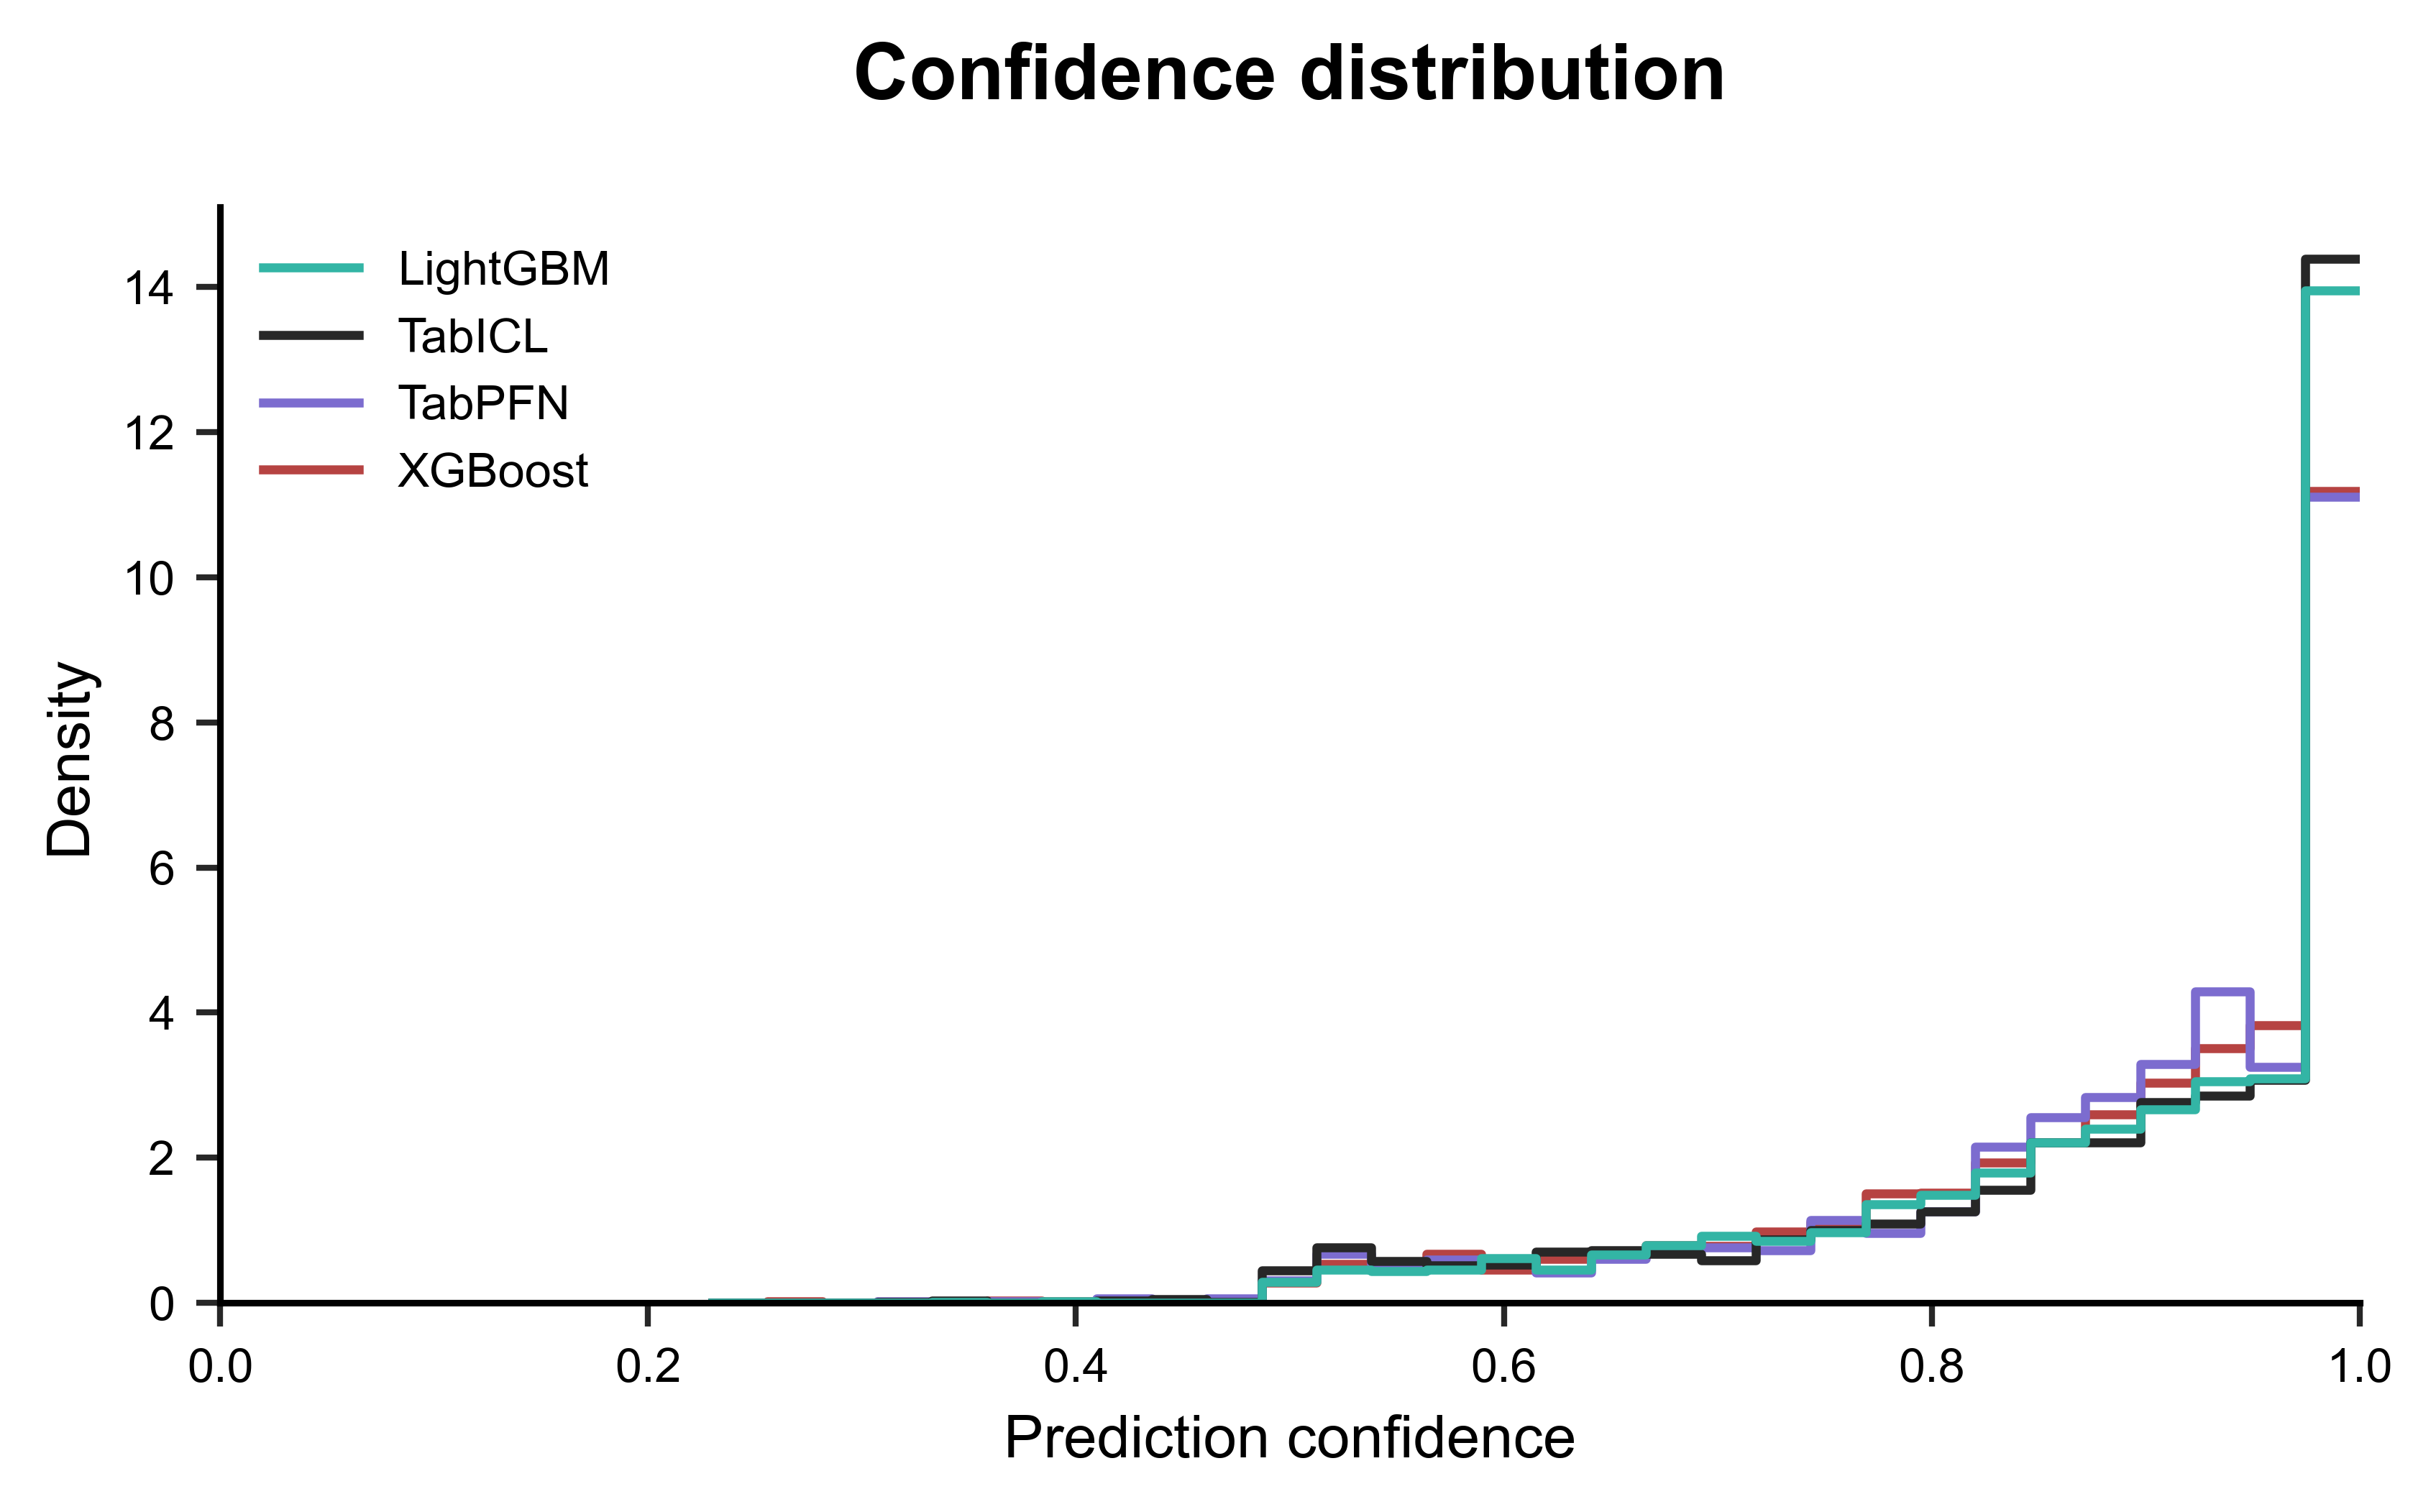
\includegraphics[width=0.5\linewidth]{figures/confidence_histogram_by_model.png}
    \caption{Enter Caption}
    \label{fig:placeholder}
\end{figure}

\subsection{Error Patterns}

For the multi-class mfeat datasets, we examine confusion matrices to identify systematic error patterns. Table X lists the most frequent off-diagonal confusions across models.
A striking cross-model pattern emerges: the digit pair 7 ↔ 10 is the dominant source of error on five of six mfeat datasets across all four models. On mfeat-morphological (6 features), LightGBM confuses true label 7 as 10 in 30 test samples and true label 10 as 7 in 26 samples—accounting for roughly half of all errors. TabICL and TabPFN exhibit the same confusion at similar magnitudes. This consistency across model families strongly suggests that the confusion arises from the feature representation rather than from any model-specific weakness: with only 6 morphological features, digits 7 and 10 appear visually similar in feature space.
The confusion largely disappears when feature dimensionality increases. On mfeat-pixel (240 features), the 7↔10 confusion drops to just 1–3 samples per model, and overall accuracy rises above 0.96. This confirms that richer feature representations resolve the ambiguity that plagues low-dimensional mfeat variants.
Other consistent confusions include 4↔5, 4↔6, and 6↔4, though at lower frequencies. These too diminish as feature count increases.

\begin{figure}
    \centering
    
\includegraphics[width=0.5\linewidth]{confusion_matrix_tabicl_mfeat-pixel_2000rows_240feat_multiclass.png}
    \caption{Enter Caption}
    \label{fig:placeholder}
\end{figure}

\begin{figure}
    \centering
    
\includegraphics[width=0.5\linewidth]{confusion_matrix_tabicl_mfeat-morphological_2000rows_6feat_multiclass.png}
    \caption{Enter Caption}
    \label{fig:placeholder}
\end{figure}


%% =========================================================================

% Conclusion

%% =========================================================================

\section{Conclusion}

This study presents a systematic benchmark comparing two tabular foundation models—\texttt{TabPFN} and \texttt{TabICL}—against two established gradient-boosted baselines—\texttt{XGBoost} and \texttt{LightGBM}—across 12 \texttt{TALENT} classification datasets under a controlled-variable experimental design. Our evaluation spans four dimensions: predictive performance, computational cost, scalability, and confidence calibration.

\textbf{Predictive performance.} Both tabular foundation models (TFMs) achieve superior average Macro-F1 compared to tree baselines, with \texttt{TabICL} leading at 0.851 (vs.\ \texttt{LightGBM} at 0.824). However, the advantage is not universal: on easy binary tasks all models perform similarly, and on severely imbalanced datasets (\texttt{jm1}, \texttt{default\_of\_credit\_card\_clients}) all struggle comparably. The TFM advantage is most meaningful on medium-complexity multi-class tasks such as the \texttt{mfeat} series.

\textbf{Computational cost.} The accuracy gains of TFMs come at a substantial price. On the largest dataset (30,000 samples), \texttt{TabPFN} predict time exceeds 4,000 seconds on a gaming laptop, while \texttt{LightGBM} completes inference in 22 milliseconds—a five-order-of-magnitude gap. \texttt{TabICL} is faster than \texttt{TabPFN} but still requires over 600 seconds on the same dataset. Peak memory consumption tells a similar story: \texttt{TabICL} reaches 18.8 GB on the largest dataset, while tree baselines remain under 250 MB throughout.

\textbf{Scalability.} The controlled-variable design reveals that TFMs scale substantially worse than tree baselines along both sample-size and feature-count dimensions. \texttt{TabPFN}'s predict-time scalability exponent $\alpha \approx 1.6$ indicates super-linear growth with sample size; \texttt{TabICL} is somewhat better at $\alpha \approx 1.4$, but both are far above the sub-linear scaling of \texttt{LightGBM} ($\alpha \approx 0.45$) and \texttt{XGBoost} ($\alpha \approx 0.37$). Feature-count scaling exhibits a similar pattern, though at lower absolute cost. Tree baselines are effectively insensitive to feature dimensionality in the tested range.

\textbf{Confidence calibration.} All four models exhibit suboptimal calibration: correct predictions receive higher confidence than incorrect ones, but wrong predictions routinely carry non-trivial confidence. No model provides a reliable low-confidence signal for its errors. This is a shared limitation across both paradigms and represents a practical risk for deployment in high-stakes applications.

\textbf{Error patterns.} Cross-model analysis reveals that dominant error modes on \texttt{mfeat} datasets are shared by all models and driven by limited feature information rather than architecture, which largely disappear with increasing feature dimensionality.

\textbf{Limitations.} This study is limited to classification tasks without hyperparameter tuning, uses consumer-grade hardware, and the dataset selection is representative rather than exhaustive.

\textbf{Future work.} Future directions include regression and missing-value robustness experiments, retrieval-based in-context learning, and GPU performance evaluation.

Overall, our findings highlight the fundamental trade-off between predictive capability and operational efficiency in modern tabular modeling, providing clear guidance for practitioners selecting appropriate methods for different application scenarios.






% =============================================
% Part 5： 参考文献
% =============================================
%在reference.bib文件中填写参考文献，此处自动生成

\newpage
\printbibliography[title={Reference}]

\end{document}
